\documentclass[pdf]{beamer}
%\mode<presentation>{}

\usepackage{amssymb,amsmath,amsthm,enumerate,mathtools}
\usepackage[utf8]{inputenc}
\usepackage{array}
\newcolumntype{C}[1]{>{\centering\arraybackslash}m{#1}}

\usepackage{verbatim}
\usepackage[parfill]{parskip}
\usepackage{graphicx}
\usepackage{caption}
\captionsetup[figure]{labelformat=empty}
\usepackage{subcaption}
\usepackage{bm}
\usepackage{amsfonts,amscd}
%\usepackage{gensymb}
\usepackage[]{units}
\usepackage{listings}
\usepackage{multicol}
\usepackage{tcolorbox}
\usepackage{physics}
\usepackage{multirow}
\usepackage{pgfplots}
\pgfplotsset{compat=1.7}
\usepackage{hyperref}
\hypersetup{
    colorlinks=true,
    linkcolor=franklinblue,
    filecolor=magenta,      
    urlcolor=cyan,
    bookmarks=true,
    citecolor= black
    % pdftitle={Overleaf Example},
    % pdfpagemode=FullScreen,
    }
\usepackage{colortbl}
\usepackage{booktabs}
\usepackage{gensymb}
\usepackage{color}
\usepackage{natbib}

\usepackage{tikz}
\usepackage{fixltx2e}
\usepackage[english]{babel}
\usepackage[absolute,overlay]{textpos}
%\usepackage{gnuplottex} % For t-distribution using gnuplot.
%The following function is use in students t distribution. 
% \def\btextttasefunc{    gamma((\n+1)/2.)/(sqrt(\n*pi)*gamma(\n/2.))*((1+(x*x)/\n)^(-(\n+1)/2.))}    
% \def\n{7}
%\usepackage{tkz-fct} % For t-distribution plotting.
% \usepackage{pst-func} % For t-distribution plotting.
\usepackage{longtable}
\usepackage{changepage} 

\usetikzlibrary{shapes,decorations,arrows,calc,arrows.meta,fit,positioning}
\tikzset{
    -Latex,auto,node distance =1 cm and 1 cm,semithick,
    state/.style ={ellipse, draw, minimum width = 0.7 cm},
    point/.style = {circle, draw, inner sep=0.04cm,fill,node contents={}},
    bidirected/.style={Latex-Latex,dashed},
    el/.style = {inner sep=2pt, align=left, sloped}
}

%Normal Distribution
\pgfmathdeclarefunction{gauss_}{2}{\pgfmathparse{1/(#2*sqrt(2*pi))*exp(-((x-#1)^2)/(2*#2^2))}%
}
%Gamma Distribution
\pgfmathdeclarefunction{gammaPDF}{2}{
\pgfmathparse{1/(#2^#1*gamma(#1))*x^(#1-1)*exp(-x/#2)}
}

%%%%% For https://tikz.net/gaussians/ %%%%%

\usepackage{amsmath} % for \dfrac
\usepackage{tikz}
\tikzset{>=latex} % for LaTeX arrow head
\usepackage{pgfplots} % for the axis environment
\usepackage{xcolor}
\usepackage[outline]{contour} % halo around text
\contourlength{1.2pt}
\usetikzlibrary{positioning,calc}
\usetikzlibrary{backgrounds}% required for 'inner frame sep'
%\usepackage{adjustbox} % add whitespace (trim)

% define gaussian pdf and cdf
\pgfmathdeclarefunction{gauss}{3}{%
  \pgfmathparse{1/(#3*sqrt(2*pi))*exp(-((#1-#2)^2)/(2*#3^2))}%
}
\pgfmathdeclarefunction{cdf}{3}{%
  \pgfmathparse{1/(1+exp(-0.07056*((#1-#2)/#3)^3 - 1.5976*(#1-#2)/#3))}%
}
\pgfmathdeclarefunction{fq}{3}{%
  \pgfmathparse{1/(sqrt(2*pi*#1))*exp(-(sqrt(#1)-#2/#3)^2/2)}%
}
\pgfmathdeclarefunction{fq0}{1}{%
  \pgfmathparse{1/(sqrt(2*pi*#1))*exp(-#1/2))}%
}

\colorlet{mydarkblue}{blue!30!black}

% to fill an area under function
\usepgfplotslibrary{fillbetween}
\usetikzlibrary{patterns}
\pgfplotsset{compat=1.12} % TikZ coordinates <-> axes coordinates
% https://tex.stackexchange.com/questions/240642/add-vertical-line-of-equation-x-2-and-shade-a-region-in-graph-by-pgfplots

% plot aspect ratio
%\def\axisdefaultwidth{8cm}
%\def\axisdefaultheight{6cm}

% number of sample points
\def\N{50}

%%%%% End for https://tikz.net/gaussians/ %%%%%

\setbeamertemplate{caption}[numbered]

%new commands
\newcommand{\der}[2]{\frac{d#1}{d#2}}
\newcommand{\nder}[3]{\frac{d^#1 #2}{d #3 ^ #1}}
\newcommand{\pder}[2]{\frac{\partial #1}{\partial #2}}
\newcommand{\npder}[3]{\frac{\partial ^#1 #2}{\partial #3^#1}}
\newcommand{\sentencelist}{def}
\newcommand{\overbar}[1]{\mkern 1.5mu\overline{\mkern-1.5mu#1\mkern-1.5mu}\mkern 1.5mu}
\newcommand{\lined}{\overbar}
\newcommand{\perm}[2]{{}^{#1}\!P_{#2}}
\newcommand{\comb}[2]{{}^{#1}C_{#2}}
\newcommand{\intall}{\int_{-\infty}^{\infty}}
\newcommand{\Var}[1]{\text{Var}\left(#1\right)}
\newcommand{\E}[1]{\text{E}\left(#1\right)}
\newcommand{\define}{\equiv}
\newcommand{\diff}[1]{\mathrm{d}#1}
\newcommand{\empy}[1]{{\color{cadetblue}\texttt{#1}}}
\newcommand{\empr}[1]{{\color{franklinblue}\textbf{#1}}}
%https://tex.stackexchange.com/questions/192358/quickly-changing-all-the-file-paths-in-a-tex-file
%\newcommand{\pathtopdf}{C:/Users/bkwei/OneDrive - Franklin University/Desktop/Math_215/Data/IMDB/Processed} - Not Tested!
\newcolumntype{L}[1]{>{\raggedright\let\newline\\\arraybackslash\hspace{0pt}}m{#1}}
\newcolumntype{C}[1]{>{\centering\let\newline\\\arraybackslash\hspace{0pt}}m{#1}}
\newcolumntype{R}[1]{>{\raggedleft\let\newline\\\arraybackslash\hspace{0pt}}m{#1}}

\theoremstyle{remark}
\newtheorem*{remark}{Remark}
\theoremstyle{definition}

\newcommand{\examplebox}[2]{
\begin{tcolorbox}[colframe=darkcardinal,colback=boxgray,title=#1]
\end{tcolorbox}}

\newcommand{\eld}[1]{\frac{d}{dt}(\frac{\partial L}{\partial \dot #1}) - \frac{\partial L}{\partial #1}=0}
\newcommand{\euler}[1]{\frac{\partial L}{\partial #1}-\frac{d}{dt}(\frac{\partial L}{\partial \dot #1})}
\newcommand{\eulerg}[1]{\frac{\partial g}{\partial #1}-\frac{d}{dt}(\frac{\partial g}{\partial \dot #1})}
\newcommand{\divg}[1]{\nabla\cdot #1}
\newcommand{\prob}[1]{P(#1\vert I)}

\AtBeginSection[]{
  \begin{frame}
  \vfill
  \centering
  \begin{beamercolorbox}[sep=8pt,center,%shadow=true,
  rounded=true]{section}
    \LARGE
    \usebeamerfont{section}
    %\usebeamercolor[fg]{section}\inserttitle %\insertsectionhead\par%
    \setbeamercolor{section}{fg=white,bg=white}\insertsectionhead\par%
  \end{beamercolorbox}
  \vfill
  \end{frame}
}

\usetheme{Franklin} 
\def \i  {\item}
\def \ai {\item[] \quad \arrowbullet}
\newcommand \si[1]{\item[] \quad \bulletcolor{#1}}
\def \wi {\item[] \quad $\ \phantom{\Rightarrow}\ $}
\def \bi {\begin{itemize}\item}
\def \ei {\end{itemize}}
\def \be {\begin{equation*}}
\def \ee {\end{equation*}}
\def \bie {$\displaystyle{}
\def \eie {{\ }$}}
\def \bsie {\small$\displaystyle{}
\def \esie {{\ }$}\normalsize\selectfont}
\def \bse {\small\begin{equation*}}
\def \ese {\end{equation*}\normalsize}
\def \bfe {\footnotesize\begin{equation*}}
\def \efe {\end{equation*}\normalsize}
\renewcommand \le[1] {\\ \medskip \lefteqn{\hspace{1cm}#1} \medskip}
\def \bex {\begin{example}}
\def \eex {\end{example}}
\def \bfig {\begin{figure}}
\def \efig {\end{figure}}
\def \btheo {\begin{theorem}}
\def \etheo {\end{theorem}}
\def \bc {\begin{columns}}
\def \ec {\end{columns}}
\def \btab {\begin{tabbing}}
\def \etab {\end{tabbing}\svneg\svneg}
\newcommand \col[1]{\column{#1\linewidth}}
\def\vneg  {\vspace{-5mm}}
\def\lvneg {\vspace{-10mm}}
\def\svneg {\vspace{-2mm}}
\def\tvneg {\vspace{-1mm}}
\def\vpos  {\vspace{5mm}}
\def\lvpos {\vspace{10mm}}
\def\svpos {\vspace{2mm}}
\def\tvpos {\vspace{1mm}}
\def\hneg  {\hspace{-5mm}}
\def\lhneg {\hspace{-10mm}}
\def\shneg {\hspace{-2mm}}
\def\thneg {\hspace{-1mm}}
\def\hpos  {\hspace{5mm}}
\def\lhpos {\hspace{10mm}}
\def\shpos {\hspace{2mm}}

\logo{
\includegraphics[height=0.4in]{./style_files_franklin/FranklinUniversity_TM1.jpg}}

\title{BUSA 603}
\subtitle{Module 5:   Marketing Mix Models}

\beamertemplatenavigationsymbolsempty

\begin{document}

\author[B. Weikel, Franklin University]{
	\begin{tabular}{c} 
	\Large
	Brian Weikel\\
    \footnotesize \href{mailto:brian.weikel@franklin.edu}{brian.weikel@franklin.edu}
    \vspace{1ex}
\end{tabular}
\vspace{-4ex}}

\institute{
	
\includegraphics[height=0.4in]{./style_files_franklin/FranklinUniversity_TM1.jpg}\\
	Business Analytics\\
	Franklin University}

\date{Spring 2024}%{\today}

\begin{noheadline}
\begin{frame}[t]\maketitle\end{frame}
\end{noheadline}

\begin{frame}[t]{Outline\footnote{These lecture notes map to chapters 14 and 15 of \cite{davis2022}.}}
\begin{enumerate}
\item  The Concept of Marketing Mix
\vspace{1.5ex}
\item  Model Specifications, Diagnostics and Fit
\vspace{1.5ex}
\item  Media Planning
\vspace{1.5ex}
\item Patterns of Advertising Response, Wear-In, Wear-Out and Response Curves 
\vspace{1.5ex}
\item Synergy Measurement via Moderation in Linear Models
\end{enumerate}
\end{frame}

\section{The Concept of Marketing Mix}

\begin{frame}[t]{The Concept of Marketing Mix}
The \empr{marketing mix} refers to variables that a marketing manager can control to influence a brand's sales or market share. Traditionally, these variables are a subset of the 4 P's or 7 P's.\footnote{See Module 1 for the definition of each P.  As mentioned in Module 4, a particular item's regular price and clearance price are almost always determined by the finance department of a company.} \\
\vspace{1.5ex}
The perennial question that managers face is, what level or combination of these variables maximizes sales, market share, or profit? \\
\vspace{1.5ex}
 The answer to this question, in turn, depends on the following question: How do sales or market share respond to past levels of  expenditures on these variables? Researchers, industry practitioners and data scientists have focused intently on trying to find answers to this question. 
\end{frame}

\begin{frame}[t]{Marketing Mix Modeling}
To address the question, they have developed a variety of market response econometric models.  Unsurprisingly, they are referred to as \empr{marketing mix models} (MMM).\footnote{Beyond the textbook of the course, other MMM introductions are \cite{tellis2006} and \cite{solana2014}.} \\
\vspace{1.5ex}
MMM, the use of statistical analysis to estimate the past impact and predict the future impact of various marketing tactics on sales, can deeply inform marketing plans. \\
\vspace{1.5ex}
While marketing spend and bottom line results are often perceived as disconnected by marketing professionals, MMM closes the loop and may be used to improve the return on marketing investment (ROMI).
\end{frame}

\section{Model Specifications, Diagnostics and Fit}

\begin{frame}[t]{A Linear Model Specification}
While from a practitioner perspective there are 5 basic  different models used to model the marketing mix, we will focus on two models: the \empr{linear model} and the \empr{multiplicative model}.  The linear model takes the form \\
\vspace{-3.0ex}
\small
\begin{multline} \label{eq:1}
Y_{t} = \alpha + \sum_{i=1}^{I}\beta_{1i} A_{it} + \sum_{j=1}^{J}\beta_{2j} P_{jt} + \sum_{k=1}^{K}\beta_{3k}R_{kt} \\ 
 + \sum_{l=1}^{L}\beta_{4l}Q_{lt} + \sum_{m=1}^{M}\beta_{5m}X_{mt} + \epsilon_t,
 \end{multline}
 \normalsize
where:
\vspace{-1.5ex}
\small
\begin{enumerate}
 \item $Y_t$ is the \empr{dependent variable}, also known as the \empr{outcome variable}, \empr{response variable} or  \empr{regressand}. It may be brand gross value sales, item units, or item \empr{equivalized units}.\footnote{Equivalized units is a unit of measurement that permits items to be compared across brands and product categories.  A few examples include pounds, kilograms, gallons,  ounces, liters, doses, uses, and cases.}
\end{enumerate}
\end{frame}

\begin{frame}[t]{Independent Variables}
 \small
 \begin{enumerate}
\setcounter{enumi}{1} 
 \item The other capital Latin letters represent \empr{independent variables} of the marketing mix.
    \begin{itemize}
          \vspace{1.0ex}
          \item $I$ advertising independent variables: $A_{it}, i \in \{1,2,\ldots, I\}$.
          \vspace{1.0ex}
          \item $J$ pricing independent variables: $P_{jt}, j \in \{1,2,\ldots, J\}$.
          \vspace{1.0ex}
          \item $K$ sales promotion, merchandising, and distribution independent variables: $R_{kt}, k \in \{1,2,\ldots, K\}$.
          \vspace{1.0ex}
          \item $L$ assortment quality independent variables: $Q_{lt}, l \in \{1,2,\ldots, L\}$.
          \vspace{1.0ex}
          \item $M$ other factors, such as seasonality, competition, and economic conditions beyond the marketers control that influences sales:  $X_{mt}, m \in \{1,2,\ldots, M\}$. 
    \end{itemize} 
    Independent variables may also be called \empr{explanatory variables} or \empr{regressors}.
\end{enumerate}
\end{frame}

\begin{frame}[t]{Coefficients and Errors}
\small
 \begin{enumerate}
 \setcounter{enumi}{2} 
  \item The subscript $t$ represents time.\footnote{Implicit in the model specification is that that there is one product, one market and one customer segment, such as brand-national-all customers.  In industry practice, a more granular dependent variable and independent variables are modeled.  For example, sub-brand or price-promoted group for product. Store, sales channel (e.g., brick-and-mortar or online) or, \href{https://markets.nielsen.com/us/en/contact-us/intl-campaigns/dma-maps/}{designated market area} (DMA) in lieu of national. %\href{https://www.iriworldwide.com/en-us/insights/training/data-detective-omnimarket-core-outlets}{IRI OmniMarket Core Outlets}, \href{https://nielseniq.com/global/en/client-learning/retail-measurement-services/}{NielsenIQ ScanTrack Markets} for market, and new and existing customer segments for customer dimensions.
  }
 \item The \empr{coefficients}, $\alpha$, $\beta_{1i}, \beta_{2j}, \beta_{3k}, \beta_{4l}$, and $\beta_{5m}$ for $i \in \{1,2,\ldots, I\}, j \in \{1,2,\ldots, J\}, k \in \{1,2,\ldots, K\}, l \in \{1,2,\ldots, L\}$ and $m \in \{1,2,\ldots, M\}$,  are \empr{parameters} that the researcher wants to estimate. They represent the effect of the independent variables on the dependent variable. 
  \item The $\epsilon_t$  are \empr{errors} that are assumed be \empr{independently and identically distributed} (IID).   This assumption means that there is no pattern to the errors so that they constitute just random noise, which is referred to as \empr{white noise}.\footnote{Many times the $\epsilon_t$ are also assumed to be normally distributed.} 
\end{enumerate}
\end{frame}

\begin{frame}[t]{Multiplicative Model Specification}
The multiplicative model takes the form
\begin{multline} \label{eq:2}
Y_{t} = \exp\{\alpha\} \prod_{i=1}^{I}\ A_{it}^{\beta_{1i}} \prod_{j=1}^{J}P_{jt}^{\beta_{2j}} \prod_{k=1}^{K}R_{kt}^{\beta_{3k}} \\ 
 + \prod_{l=1}^{L}Q_{lt}^{\beta_{4l}} \prod_{m=1}^{M}X_{mt}^{\beta_{5m}} \exp\{\epsilon_t\},
 \end{multline} 
or after a  natural logarithm transformation, 
\small
\begin{multline} \label{eq:3}
\log Y_{t} = \alpha + \sum_{i=1}^{I}\beta_{1i} \log A_{it} + \sum_{j=1}^{J}\beta_{2j} \log P_{jt} + \sum_{k=1}^{K}\beta_{3k}\log R_{kt} \\ 
 + \sum_{l=1}^{L}\beta_{4l} \log Q_{lt} + \sum_{m=1}^{M}\beta_{5m} \log  X_{mt} + \epsilon_t.
 \end{multline}
 \normalsize
\end{frame}

\begin{frame}[t]{Multiplicative Model Specification Benefits}
After this transformation, the error terms in Equation \ref{eq:3} are assumed to be IID, and usually normally distributed. \\
\vspace{1.5ex}
The multiplicative model has many benefits. \\
\vspace{0.0ex}
\small
\begin{enumerate}
\item This model implies that the dependent variable is affected by an \empr{interaction} of the variables of the marketing mix. In other words, the independent variables have a \empr{synergistic effect} on the dependent variable. For example, larger advertising combined with a price decrease may enhance sales more than the sum of larger advertising or the price decrease occurring alone.
\item The multiplicative model specification implies that response of sales to any of the independent variables can take on a variety of shapes depending on the value of the coefficient.
\item The coefficients not only estimate the effects of the independent variables on the dependent variables, but they are also \empr{elasticities}.
\end{enumerate}
\end{frame}

\begin{frame}[t]{Multiplicative Model Specification Limitations}
The multiplicative model has several limitations. \\
\vspace{0.0ex}
\small
\begin{enumerate}
\item Using the natural logarithm specification implies rigidity in modeling select advertising  effects. For example, using the natural logarithm transformation results in  inflexibility in modeling the sales-advertising response shape effect.\footnote{In industry practice the natural logarithm transformation is replaced by a more flexible transformation, such as the Hill function.  For more information, see \cite{jin2017bayesian}.}
\item The multiplicative model implies that the elasticity of sales to advertising is constant. That is, the percentage change in sales for a percentage change in advertising is the same indifferent to advertising or sales levels. This result is quite implausible.
\end{enumerate}
\normalsize
\vspace{-2.0ex}
The two models are \empr{regression} models, a simple but powerful statistical methodology. 
\end{frame}

\begin{frame}[t]{Estimator and Estimate Definitions}
Regression coefficients for these these models are frequently estimated by the \empr{principle of least squares}.   \\
\vspace{1.5ex}
An \empr{estimator} is a formula, method, or recipe (e.g., numerical algorithm) for estimating an unknown \empr{population} \empr{parameter}. An \empr{estimate} is the numerical value obtained when sample data are substituted in the formula. \\
\vspace{1.5ex}
For simplicity purposes we will consider a bivariate regression specification. Let the \empr{residuals} from a \underline{fitted} straight line be,\\
\vspace{-1.0ex}
\begin{equation}
\hat{\epsilon}_i = y_i - \hat{y}_i = y_i - \hat{\beta}_0 - \hat{\beta}_1x_i, \;\; i = \{1,2,\ldots,n\}.
\end{equation}
From the definition of $\hat{y}_i$, these residuals are seen to be measured in the vertical (i.e., $y$) direction.  Different values of the intercept ($\hat{\beta}_0$) and slope ($\hat{\beta}_1$) define a  different line, and hence a different set of residuals.
\end{frame}

\begin{frame}[t]{Least-Squares Principle}
The least squares principle is to identify values for $\beta_0$ and $\beta_1$ to minimize the \empr{residual sum of squares} (RSS): \\
\vspace{-0.5ex}
\begin{equation}
\text{RSS} = \sum_{i=1}^{n} \epsilon_{i}^{2} = \sum_{i=1}^{n}(y_i-\beta_0-\beta_1x_i)^2.
\end{equation}
Upon minimizing RSS with sample data, $\beta_0$ is replaced by $\hat{\beta}_0$ and $\beta_1$ is replaced by $\hat{\beta}_1$. \\
\vspace{1.5ex} 
There are necessary conditions for a stationary value of RSS.  Using calculus, these conditions are:
\begin{equation} \label{eq:ls1}
-2 \sum_{i=1}^n(y_i-\beta_0 - \beta_1x_i) = 0, \;\; \text{and}
\end{equation}
\begin{equation} \label{eq:ls2}
-2 \sum_{i=1}^n x_i(y_i-\beta_0 - \beta_1x_i) = 0.
\end{equation}
\end{frame}

\begin{frame}[t]{Normal Equations}
Simplifying Equations (\ref{eq:ls1}) and (\ref{eq:ls2}) yields the \empr{normal equations}\footnote{Equations (\ref{eq:ls3}) and (\ref{eq:ls4}) use the word \underline{normal} due to the geometry of the least-squares principle. For additional information see \cite{johnston1997}.}
\vspace{0.0ex}
\begin{equation} \label{eq:ls3}
\sum_{i=1}^n y_i = n \beta_0 + \beta_1 \sum_{i=1}^n x_i, \;\; \text{and}
\end{equation}
\begin{equation} \label{eq:ls4}
\sum_{i=1}^n x_i y_i =\beta_0 \sum_{i=1}^n x_i + \beta_1\sum_{i=1}^n x_i^2 = 0.
\end{equation}
Rewriting Equation (\ref{eq:ls3}) and using sample data in the formulas yields $\hat{\beta}_0 = \bar{y} - \hat{\beta}_1\bar{x}$ and $\hat{\beta}_1 = r \frac{s_y}{s_x}$.  That is, the \underline{$y$-intercept} and \underline{slope}, respectively.
\end{frame}

\begin{frame}[t]{A Regression Example - Petroleum Distillate Demand}
Since the \href{https://www.federalreservehistory.org/essays/oil-shock-of-1973-74}{OPEC oil embargo of 1973} there has been a continuing controversy in the U.S. about national and state tax policy for gasoline and other petroleum distillates.  \\
\vspace{1.5ex}
Other major disruptions in the production and/or distribution of petroleum distillates include, but are not limited to:
%https://tex.stackexchange.com/questions/228271/creating-two-columns-in-beamer \\
\vspace{1.5ex}
\begin{columns}[T]
\begin{column}{0.43\textwidth}
  \begin{itemize}
    \item Iranian revolution in the late 1970s 
     \vspace{1.0ex}
    \item Iran-Iraq war in the early 1980s
     \vspace{1.0ex}
    \item Persian Gulf War in 1990
     \vspace{1.0ex}
    \item Iraqi War in 2003
  \end{itemize}
\end{column}
\begin{column}{0.43\textwidth}  %%<--- here
  \begin{itemize}
    \item Hurricanes Katrina and Rita in 2005
     \vspace{1.0ex}
    \item Hurricanes Gustav and Ike in 2008 
     \vspace{1.0ex}
    \item Arab Spring of 2011
     \vspace{1.0ex}
    \item Russia's war with Ukraine starting in 2022
  \end{itemize}  
\end{column}
\end{columns}
\end{frame}

\begin{frame}[t]{Modeling Energy Demand is An Active Field}
A crucial component of any such debate is a reliable model for demand, which by its very nature has a long, and what some may call dubious, history.\footnote{For example see \cite{sims1980}, \cite{malinvaud1981} and \cite{freedman1983}.}  \\
\vspace{1.5ex}
As may be expected, energy demand modeling is still an active field.\footnote{A recent review of hundreds of recent articles on modeling the demand for energy is \cite{verwiebe2021}.}
\vspace{1.5ex}
We will review a rather simple petroleum demand function.  It is a multiplicative regression model.
\end{frame}

\begin{frame}[t]{Data Sources}
The data was obtained from the \href{https://fred.stlouisfed.org/}{Federal Reserve Bank of St. Louis} and the \href{https://highways.dot.gov/}{Federal Highway Administration} of the U.S. Department of Transportation. The observation level is month. Variables sourced from the sites follow.\\
\vspace{0.5ex}
\small
\begin{itemize}
\item $Y$: per capita personal consumption of gasoline in gallons (at annual rates).
\item $P$: real price of a gallon of gasoline in 2012 prices; that is 1 gallon = \$3.35 at 2012 prices.\footnote{For additional information about deflating nominal values to real values see this \href{https://www.dallasfed.org/research/basics/nominal.aspx}{Federal Reserve Bank of Dallas page}.}
\item $Z$:  per capita annual personal income in 1000's of 2012 U.S. dollars.
\item $y$:  natural logarithm of $Y$.
\item $p$:  natural logarithm of $P$.
\item $z$:  natural logarithm of $Z$. 
\end{itemize}
\end{frame}

\begin{frame}[t]{Gasoline Demand is Highly Seasonal}
\begin{figure}[htbp]
  \captionsetup{justification=centering}
  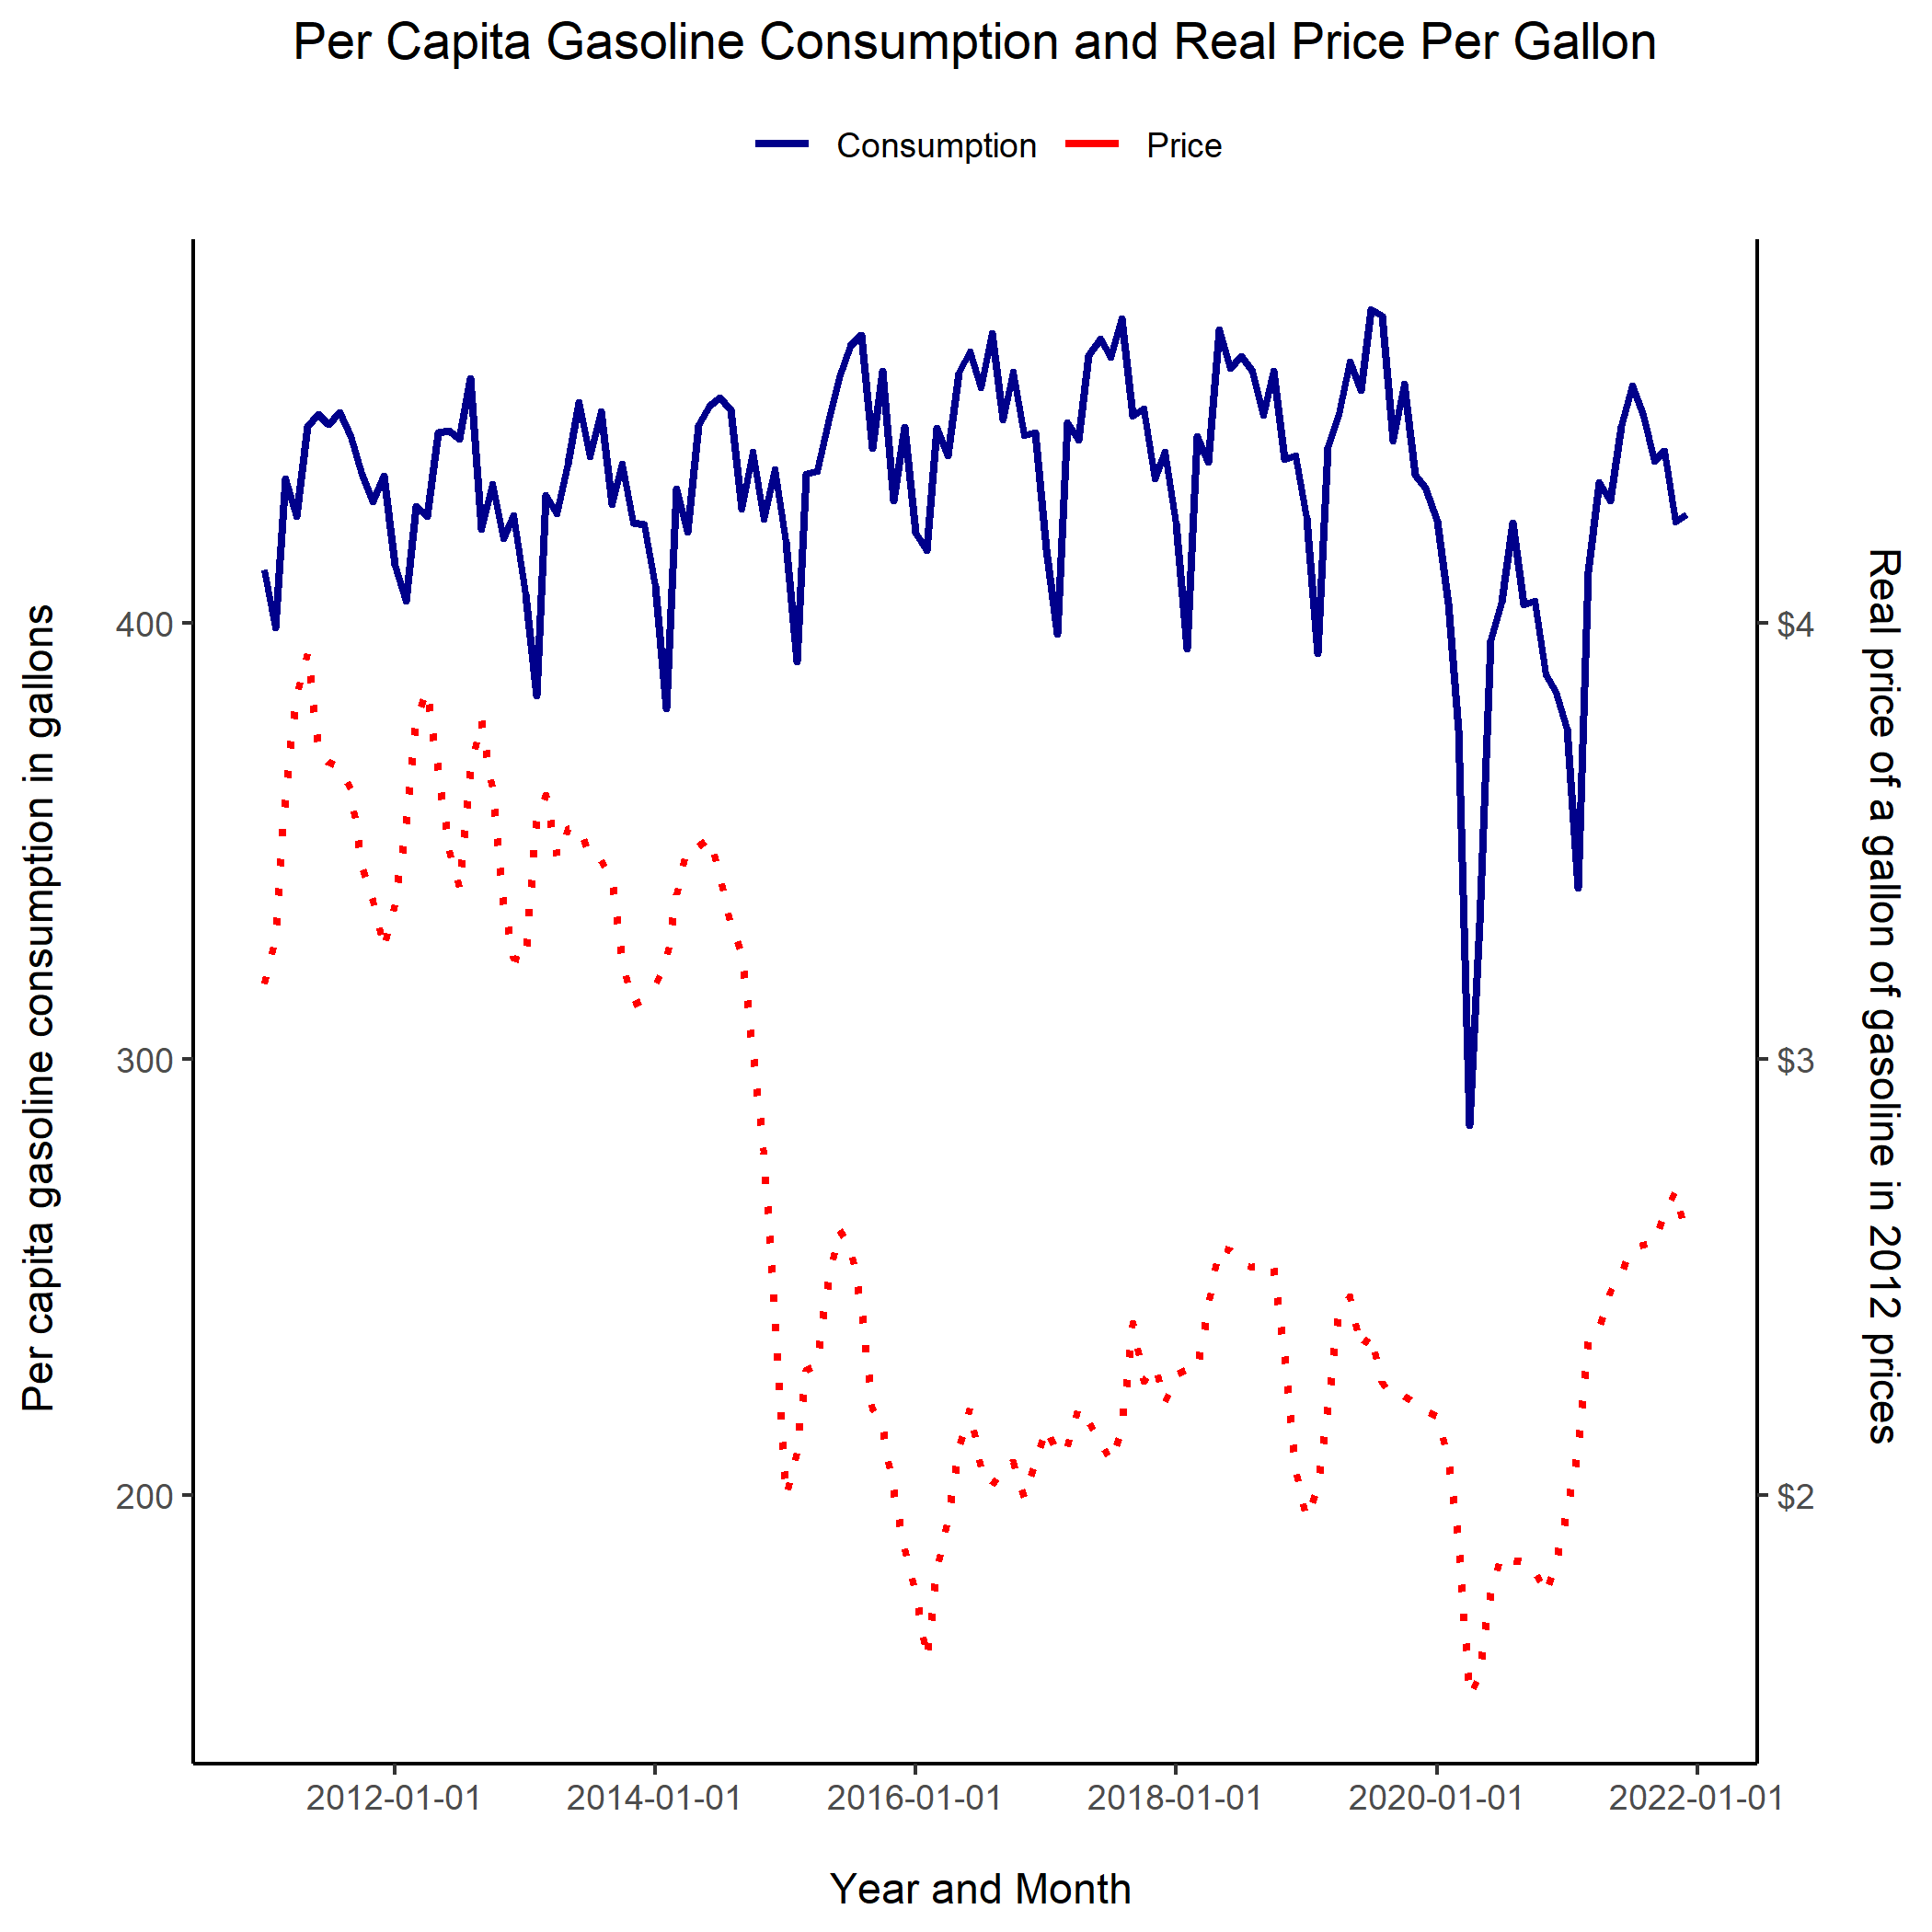
\includegraphics[height=6.8cm, trim=0.0cm 0.0cm 0.0cm 0.0cm width=6.8cm]{../BUSA_603_Gas_Demand/Data_621_A1/a1_q1a.png}
  \caption{Figure {\color{franklinblue} 1}: Gasoline Consumption and Real Price per Gallon}
\end{figure}
\end{frame}

\begin{frame}[t]{COVID-19 Produced Several Structural Breaks}
\begin{figure}[htbp]
  \captionsetup{justification=centering}
  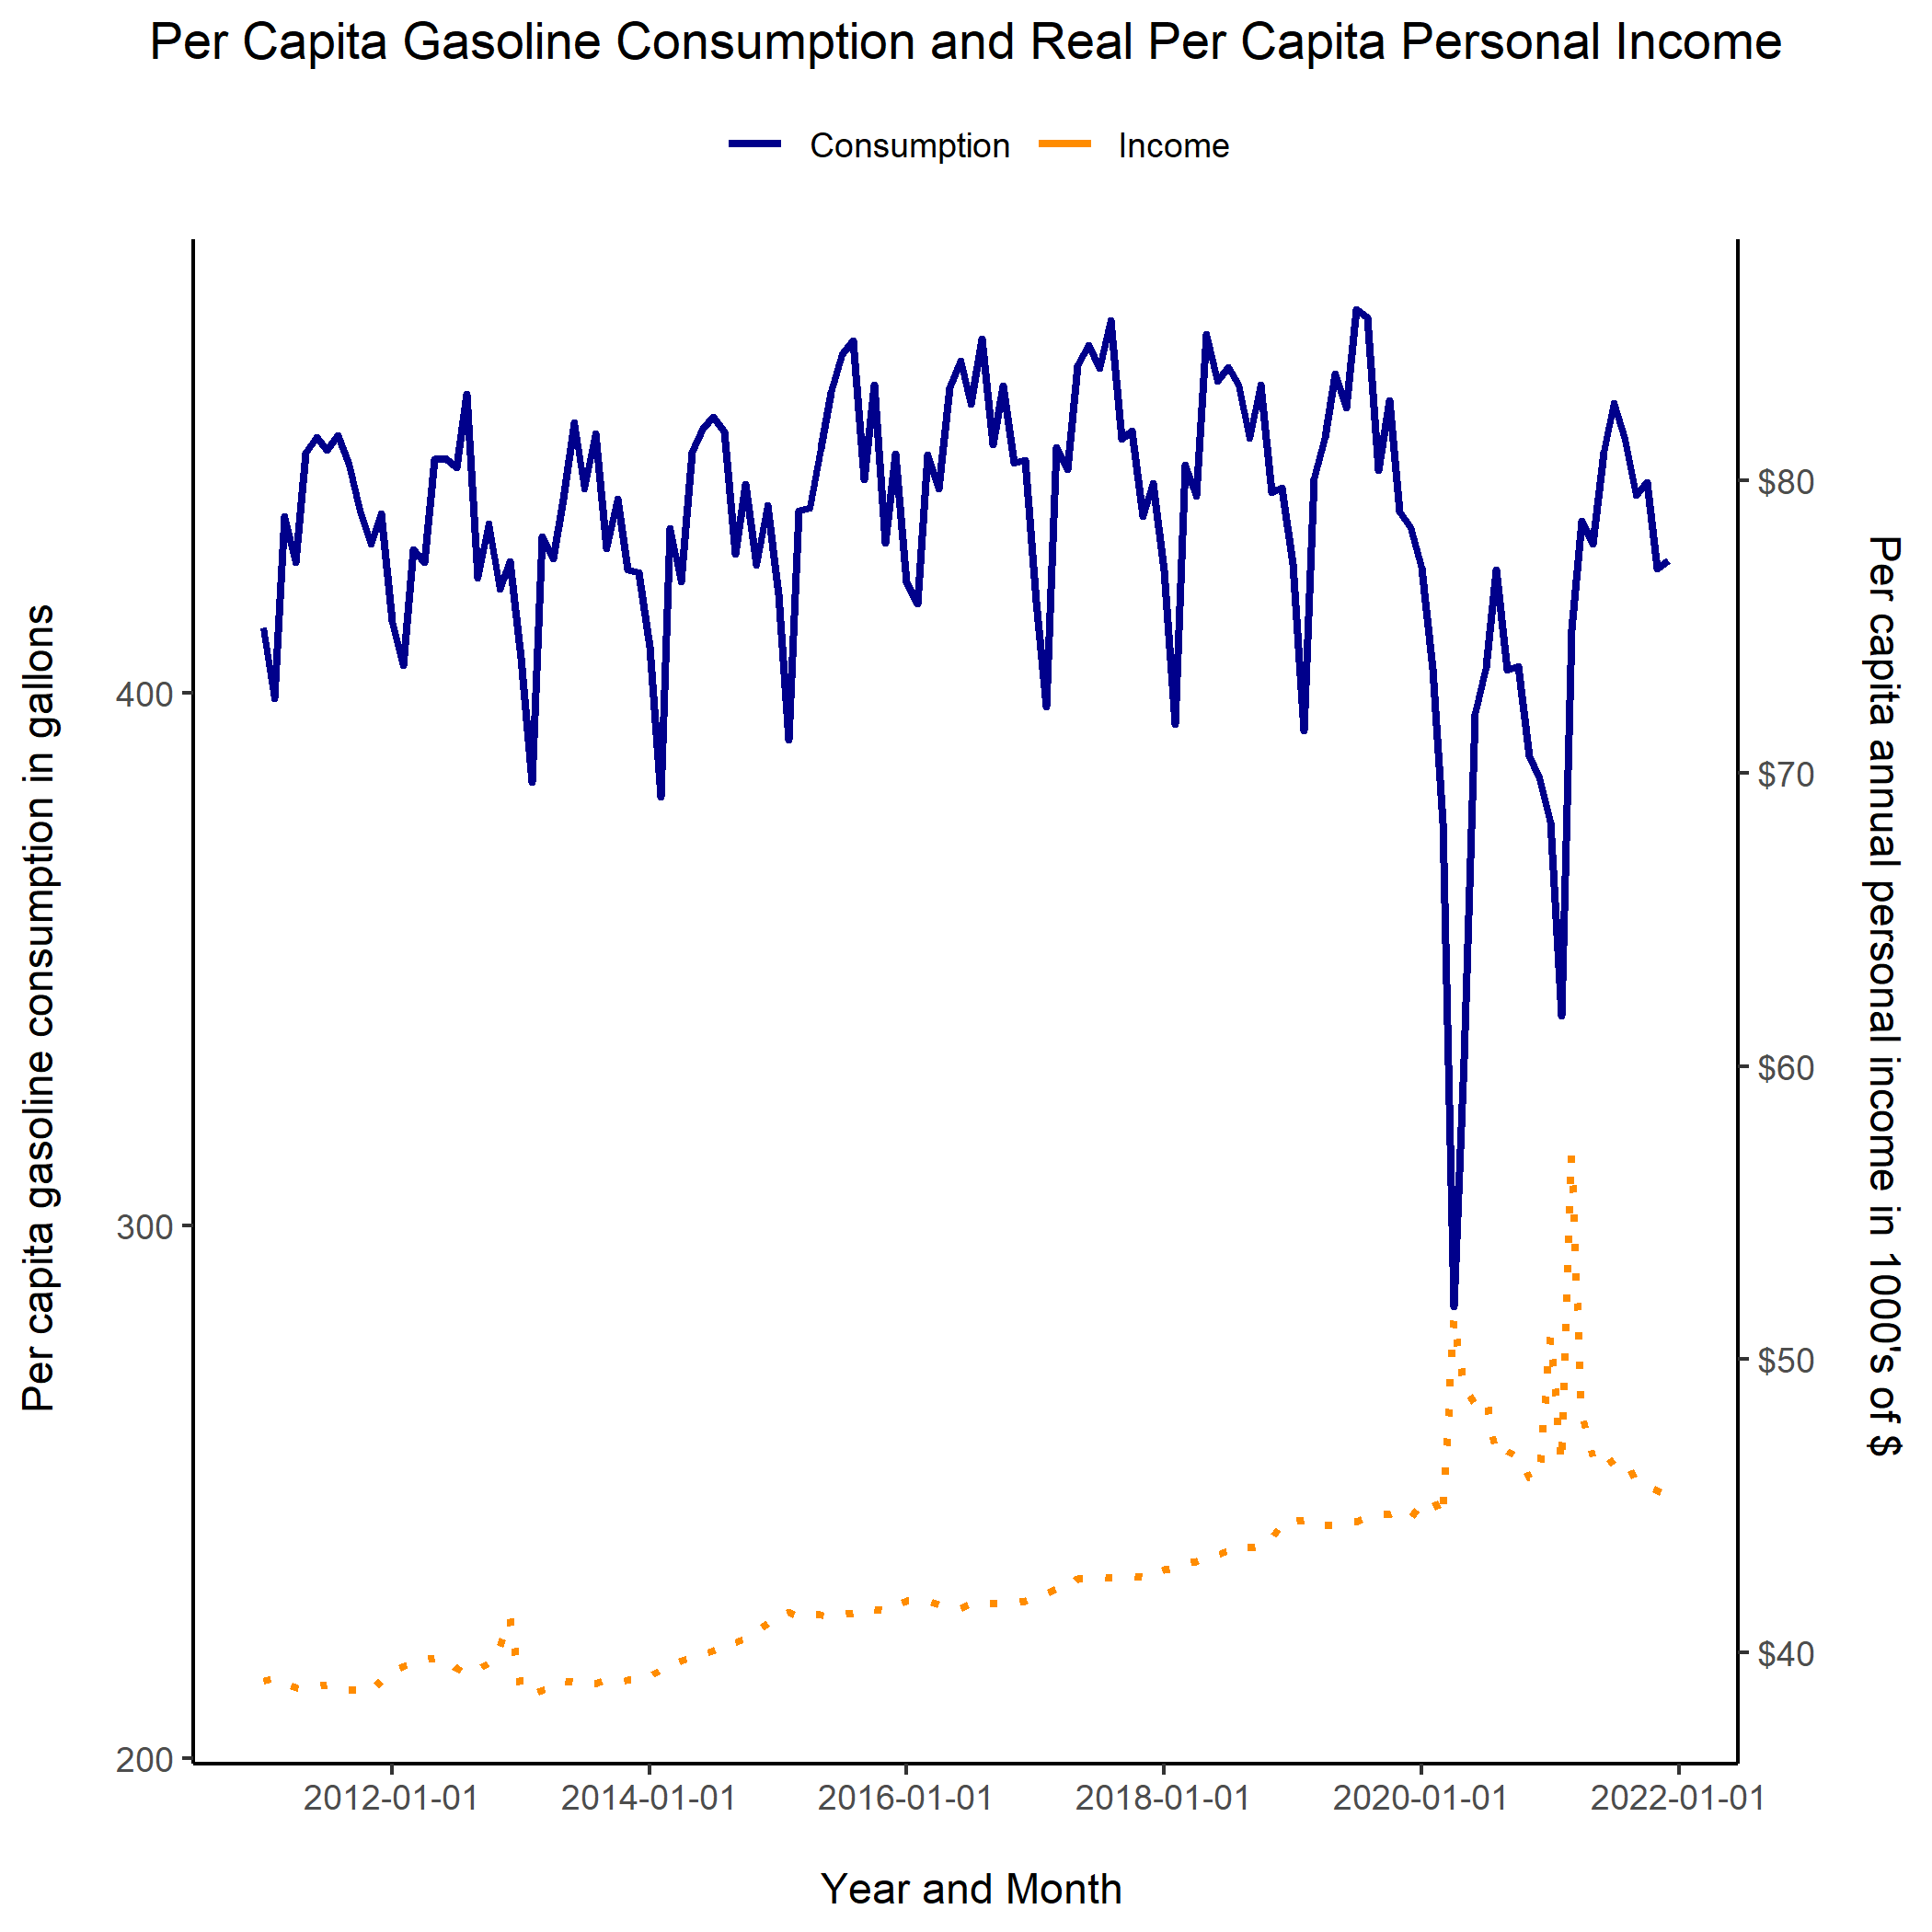
\includegraphics[height=6.8cm, trim=0.0cm 0.0cm 0.0cm 0.0cm width=6.8cm]{../BUSA_603_Gas_Demand/Data_621_A1/a1_q1b.png}
  \caption{Figure {\color{franklinblue} 2}: Gasoline Consumption and Real Per Capital Income}
\end{figure}
\end{frame}

\begin{frame}[t]{Creating a Few Explanatory Variables}
 For  $i \in \{1,2,\ldots, 12\}$, define the following monthly indicators, which will be used to model monthly demand seasonality.
    \[
    x_{it}= 
        \begin{cases}
    1,& \text{if the year of the month of observation } t \text{ is } i, \\
    0,              & \text{otherwise.}
\end{cases}
    \]
  Thus $x_{1t} = 1 $ if the month is January and 0 otherwise for observation $t$, $x_{2t} = 1 $ if the month is February and 0 otherwise for observation $t$, \ldots  \\
\vspace{1.5ex}
  To control for effects that yield a long-term trend, we will include a trend explanatory variable in our demand specification.  Let January 2010 be $t=1$.  The log trend variable is defined as $w_t = \ln(t+1), t \geq 1$.

\end{frame}

\begin{frame}[t]{Multivariate Regression Specification}
Consider the following simple equilibrium model for the demand of gasoline: \\
\vspace{-2.0ex}
    \begin{equation} \label{eqn:1}
    y_t = \beta_0 + \beta_1 z_t + \beta_2 p_t + \gamma_0w_t + \sum_{i=1}^{11}\gamma_i x_{it} + \epsilon_t.
    \end{equation}
 The errors, $\epsilon_t, t = \{1,2,\ldots,T\}$, are assumed to be IID. \\
\vspace{1.5ex}
  Since the model is specified as a log-log model in consumption, income and price, $\beta_1$ is the long-run income elasticity of demand for gasoline and $\beta_2$ is the long-run price elasticity of demand for gasoline for small changes in income and price, respectively.\footnote{To illustrate the relationship between the real price of gasoline elasticity and the real price of gasoline coefficient, suppose $\beta_2 = -0.5$.  Then a 1\% increase in the real price of gasoline is expected to produce a 0.5\% decrease in the quantity demanded of gasoline.}
\end{frame}

\begin{frame}[t]{Statistical Inference and Model Diagnostics}
\small
The standard deviation of the sampling distribution of a coefficient estimate is often referred to as the \empr{standard error} of the estimate. \\
\vspace{1.5ex}
Recall the smallest significance level at which a null hypothesis can be rejected is called the \empr{probability value}, or \empr{$\mathbf{p}$-value}.\footnote{The textbook states, ``If the $p$-value is less than or equal to .05, which is a commonly accepted threshold, then it is acceptable to say the estimate is significantly different than 0, or just significant.''}\\
\vspace{1.5ex}
The \empr{F-statistic} is the value of the test statistic for the null hypothesis that all explanatory variable coefficients are zero.\\
\vspace{1.5ex} 
\empr{$\mathbf{R^2}$} measures the proportion of the total variation in the dependent variable explained by the linear 
combination of the explanatory variables.  Mathematically, it is 1 less the ratio of the RSS divided by the \empr{total sum of squares} (TSS): $R^2 = 1 - \frac{RSS}{TSS}$.  \\
\vspace{1.5ex}
For $n$ the number of observations and $k$ the number of coefficients, \empr{Adjusted $\mathbf{R^2}$} $ = 1- \frac{RSS/(n-k)}{TSS/(n-1)}$.  Thus the statistic takes explicit account of the number of explanatory variables in the regression. 

\end{frame}

\begin{frame}[t]{Output from Model Estimation via \textsf{R} \texttt{lm} Function}
\small
\verbatiminput{../BUSA_603_Gas_Demand/Data_621_A1/a1_q2a_1.txt}
\end{frame}

\begin{frame}[t]{Output from Model Estimation Continued}
\small
\verbatiminput{../BUSA_603_Gas_Demand/Data_621_A1/a1_q2a_2.txt}
\end{frame}

\begin{frame}[t]{Exponential Attraction and Multinomial Logit Models}
Other marketing model specifications include \empr{attraction models} and the \empr{multinomial logit model} (MNL).  \\
\vspace{1.5ex}
    \begin{itemize} 
      \item Attraction models are based on the premise that market response is the result of the  attractive power of a brand relative to that of other brands with which it competes.
      \small
      \begin{itemize} 
      \item The \empr{linear attraction model} specifies a brand's share of market sales as a linear function of its share of total marketing effort. 
      \item The \empr{exponential attraction model} expresses the market share of the brand as an exponential attraction of the marketing mix.
      \end{itemize}
      \normalsize
    \item The MNL results from a log-centering transformation of the exponential attraction model.\footnote{For additional information about attraction models and MNL, see \cite{cooper1988}.}
  \end{itemize}
\end{frame}

\begin{frame}[t]{Other Model Specifications}
\small
    \begin{enumerate}
      \item The \empr{Koyck model} may be considered a simple augmentation of the basic linear model, which includes the lagged dependent variable as an independent variable.
      \item The \empr{distributed lag model} is a model with multiple lagged values of both the dependent variable and the independent variables.\footnote{For additional information on the Koyck and distributed lag models see \cite{johnston1997}.}
      \item \empr{Hierarchical models} are multistage models in which coefficients (of advertising) estimated in one stage become the dependent variable in the other stage. The second stage contains the characteristics by which advertising is likely to vary in the first stage, such as ad content, medium, or campaign duration.\footnote{For additional information on hierarchical models, see \cite{tellis2000}.}
    \end{enumerate}
\end{frame}

\section{Media Planning}

\begin{frame}[t]{Basic Components of Media Plan}
Media planning involves essentially three basic activities.\footnote{A reference that has been used for years by marketers to understand the nuances of media planning is \cite{sissors2010}.}\\
\vspace{0.0ex}
\small
\begin{enumerate}
  \item \textbf{Defining the marketing problem}:   Does the firm know where the business is coming from and where the potential for increased business lies?  Does it know the markets of greatest importance and greatest opportunity?  Does it know who is most likely to buy?  Does the firm need to stimulate trial or defend a purchase? Does the firm need to reach everyone or only a selective group of consumers? How much product loyalty exists?
  \item \textbf{Translating marketing requirements into actionable media objects}: If the marketing objective is to stimulate trial among all potential consumers, then reaching many people is more important than reaching fewer people more frequently. If the product is purchased often, then reaching people more frequently might be a more appropriate tactic.
\end{enumerate}
\end{frame}

\begin{frame}[t]{Formulating Media Strategies}
\small
\begin{enumerate}
  \setcounter{enumi}{2}
   \item  \textbf{Defining a media solution by formulating media strategies}:  If reaching people is a primary objective, one should select affordable media that will generate more reach than other media forms.  If a specific demographic group is to be reached, then media selection should be based on reaching the group effectively and efficiently. 
\end{enumerate}
\vspace{-0.5ex}
\normalsize
The objective of any media plan results in defining \empr{media goals}.  Goals must be positive, action-oriented statements representing an extension of the \empr{marketing objectives} and hence, must also be marketing-goal oriented. A few example goals follow. \\
\vspace{0.5ex}
\small
\begin{enumerate}
  \item Reach at least 80\% of the potential market within the first month of advertising, ensuring that the average consumer will be exposed to a minimum of 3 advertising messages.
  \item Direct advertising to current and potential purchasers of Product Line Z by weighting current purchasers characteristics by 60\% and potential characteristics by 40\%.
\end{enumerate}
\end{frame}

\begin{frame}[t]{Media Strategies}
\empr{Media strategies} are the solutions to the media objectives.  Strategy statements reflect the specific course to be taken with media. \\ 
\vspace{1.5ex}
\begin{enumerate}
  \item Which media will be used?
  \item How often will each be used?
  \item How much of each media will be used?
  \item During which periods of the year? 
\end{enumerate}
\end{frame}

\begin{frame}[t]{Media Strategy Scheduling Objective}
Every media plan should have a scheduling objective to guide the planner in allocating media across the year.  \\
\vspace{1.5ex}
Beyond the general timing considerations, the media planner should also consider the strategy of flighting versus continuity.  \\
\vspace{1.5ex}
\begin{itemize}
  \item \empr{Flighting} refers to periodic waves of advertising interspersed with periods of complete and absolute inactivity.
  \item \empr{Continuous} advertising is a schedule with little or no variation in activity.
  \item  \empr{Pulsing} is a combination of the above two concepts.  A continuous base of support augmented by intermittent bursts of heavy activity. 
\end{itemize} 
\end{frame}

\begin{frame}[t]{Flighting}
\begin{figure}[htbp]
  \captionsetup{justification=centering}
  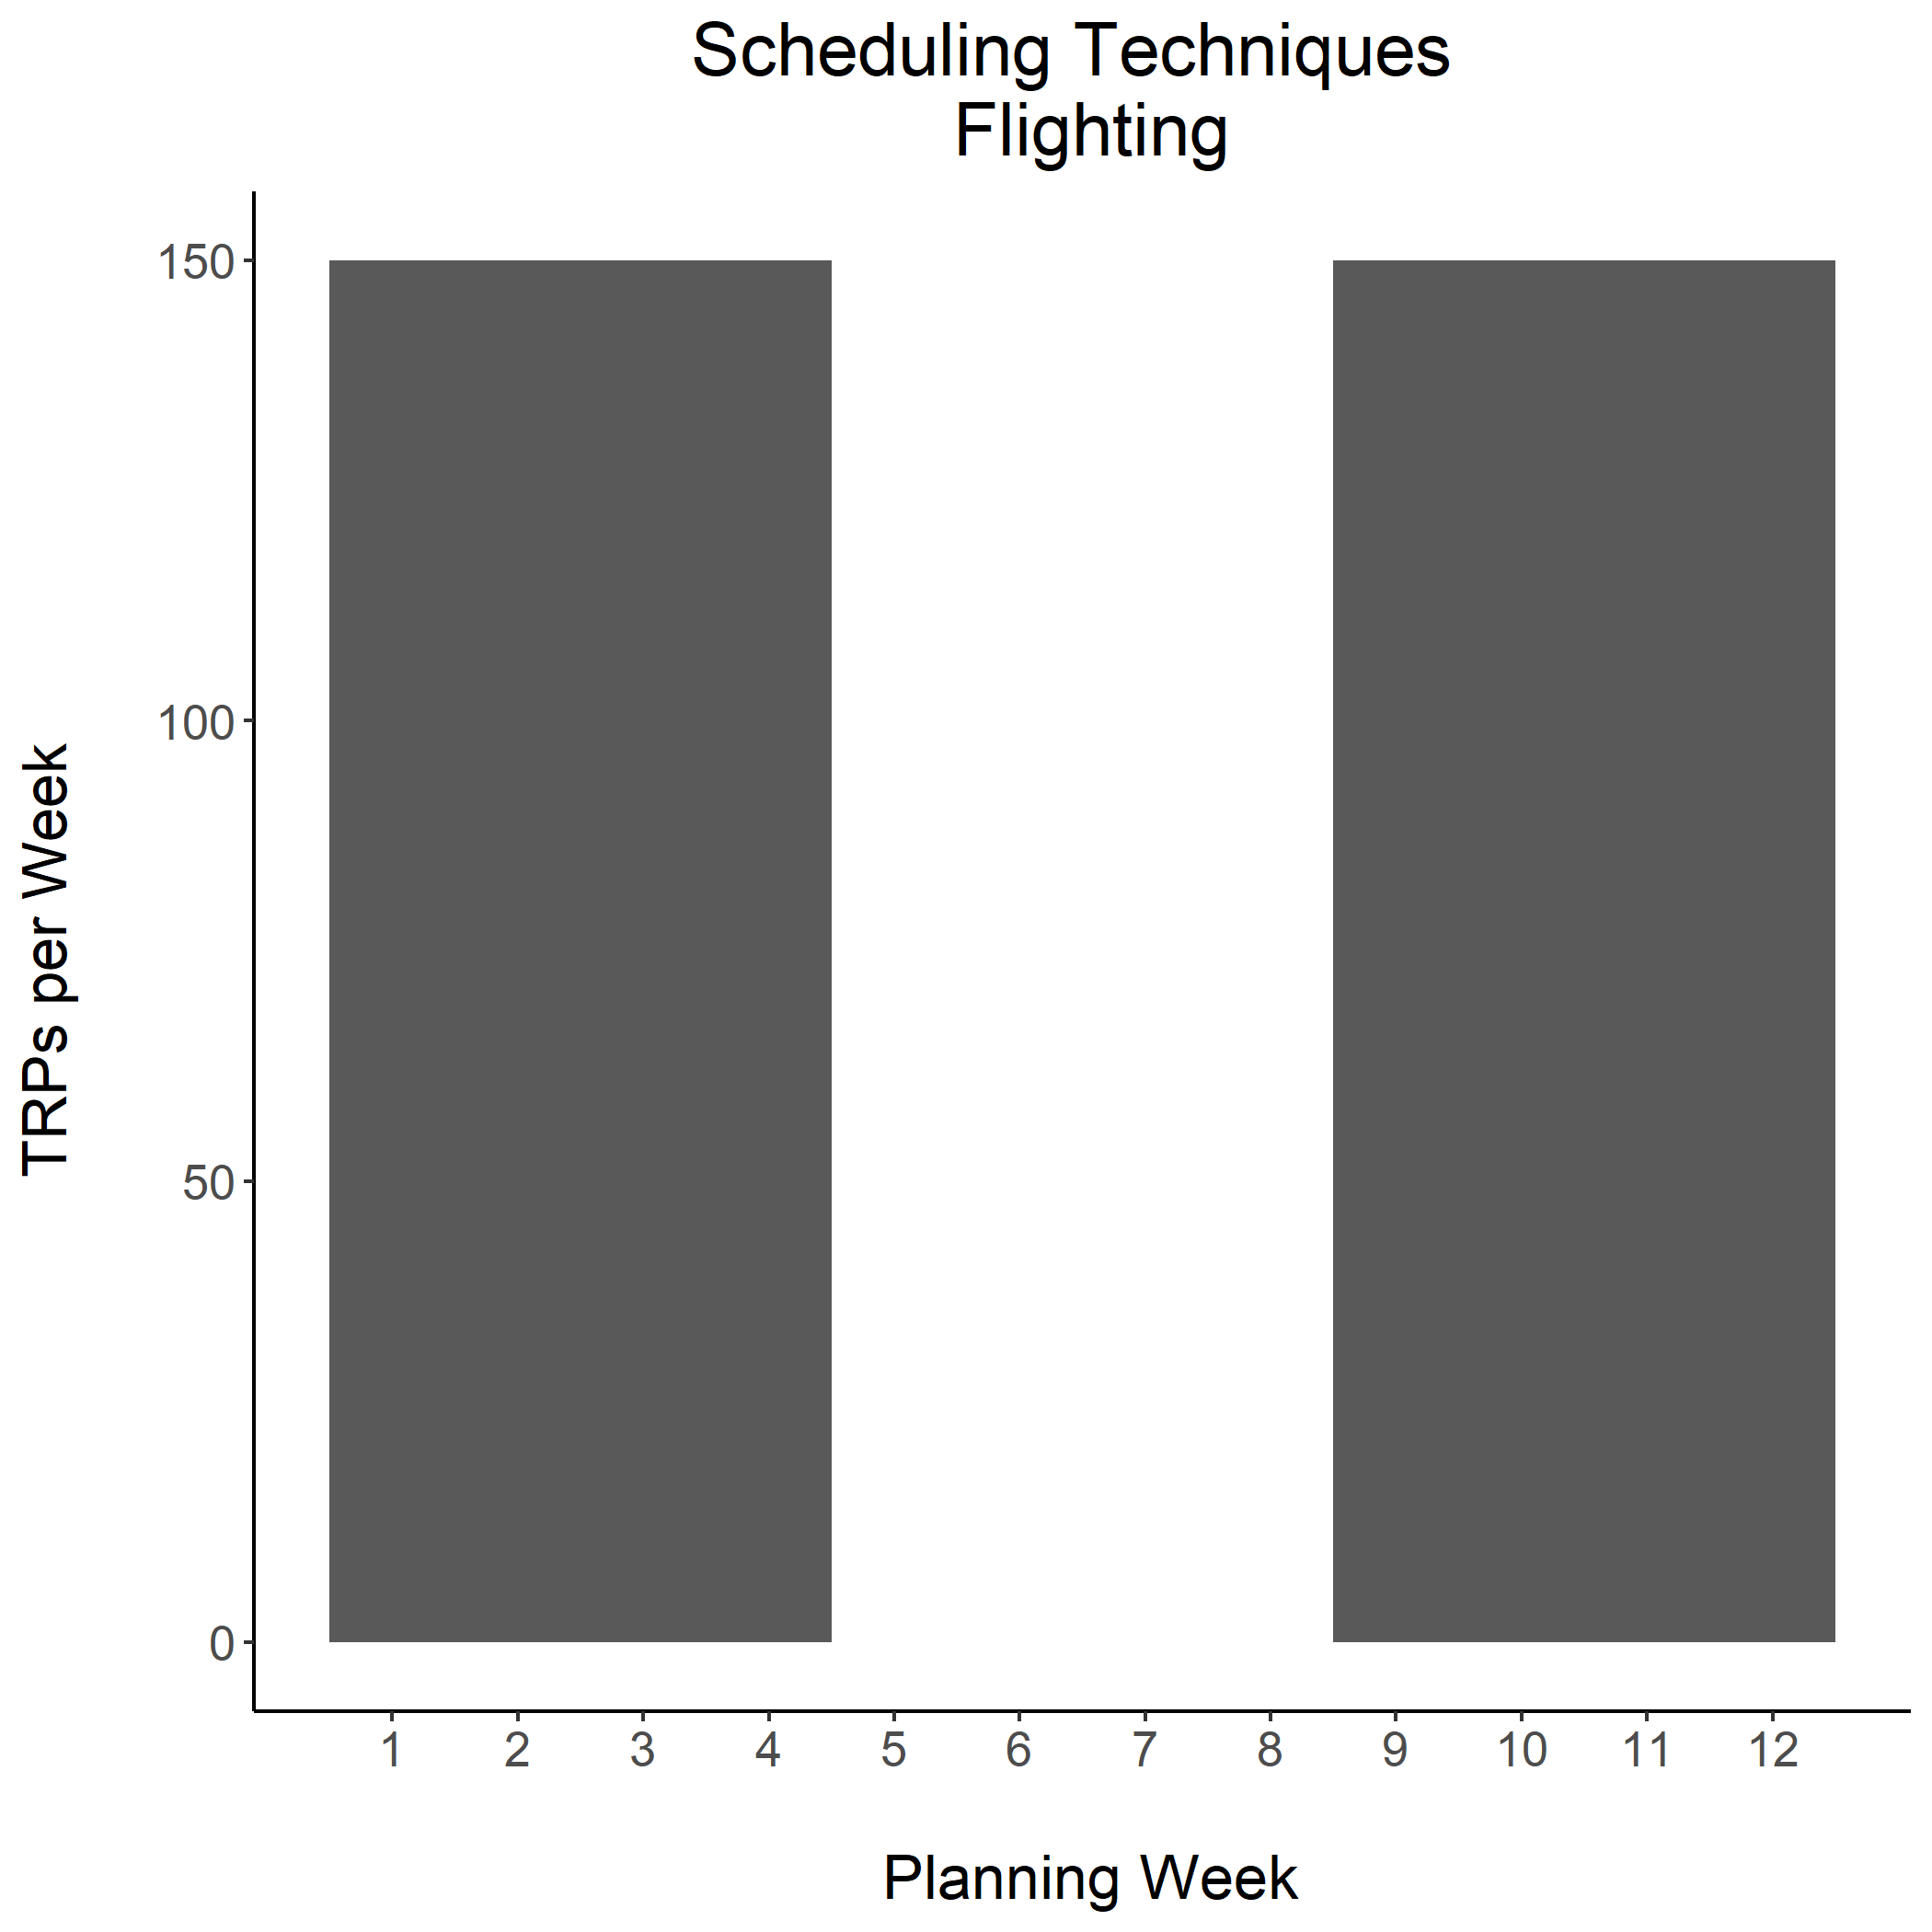
\includegraphics[height=6.8cm, trim=0.3cm 0.3cm 0.3cm 0.3cm width=6.8cm]{../BUSA_603_Ad_Response/Output/m5_0_a.png}
  \caption{Figure {\color{franklinblue} 3}: Flighting}
\end{figure}
\end{frame}

\begin{frame}[t]{Continuity}
\begin{figure}[htbp]
  \captionsetup{justification=centering}
  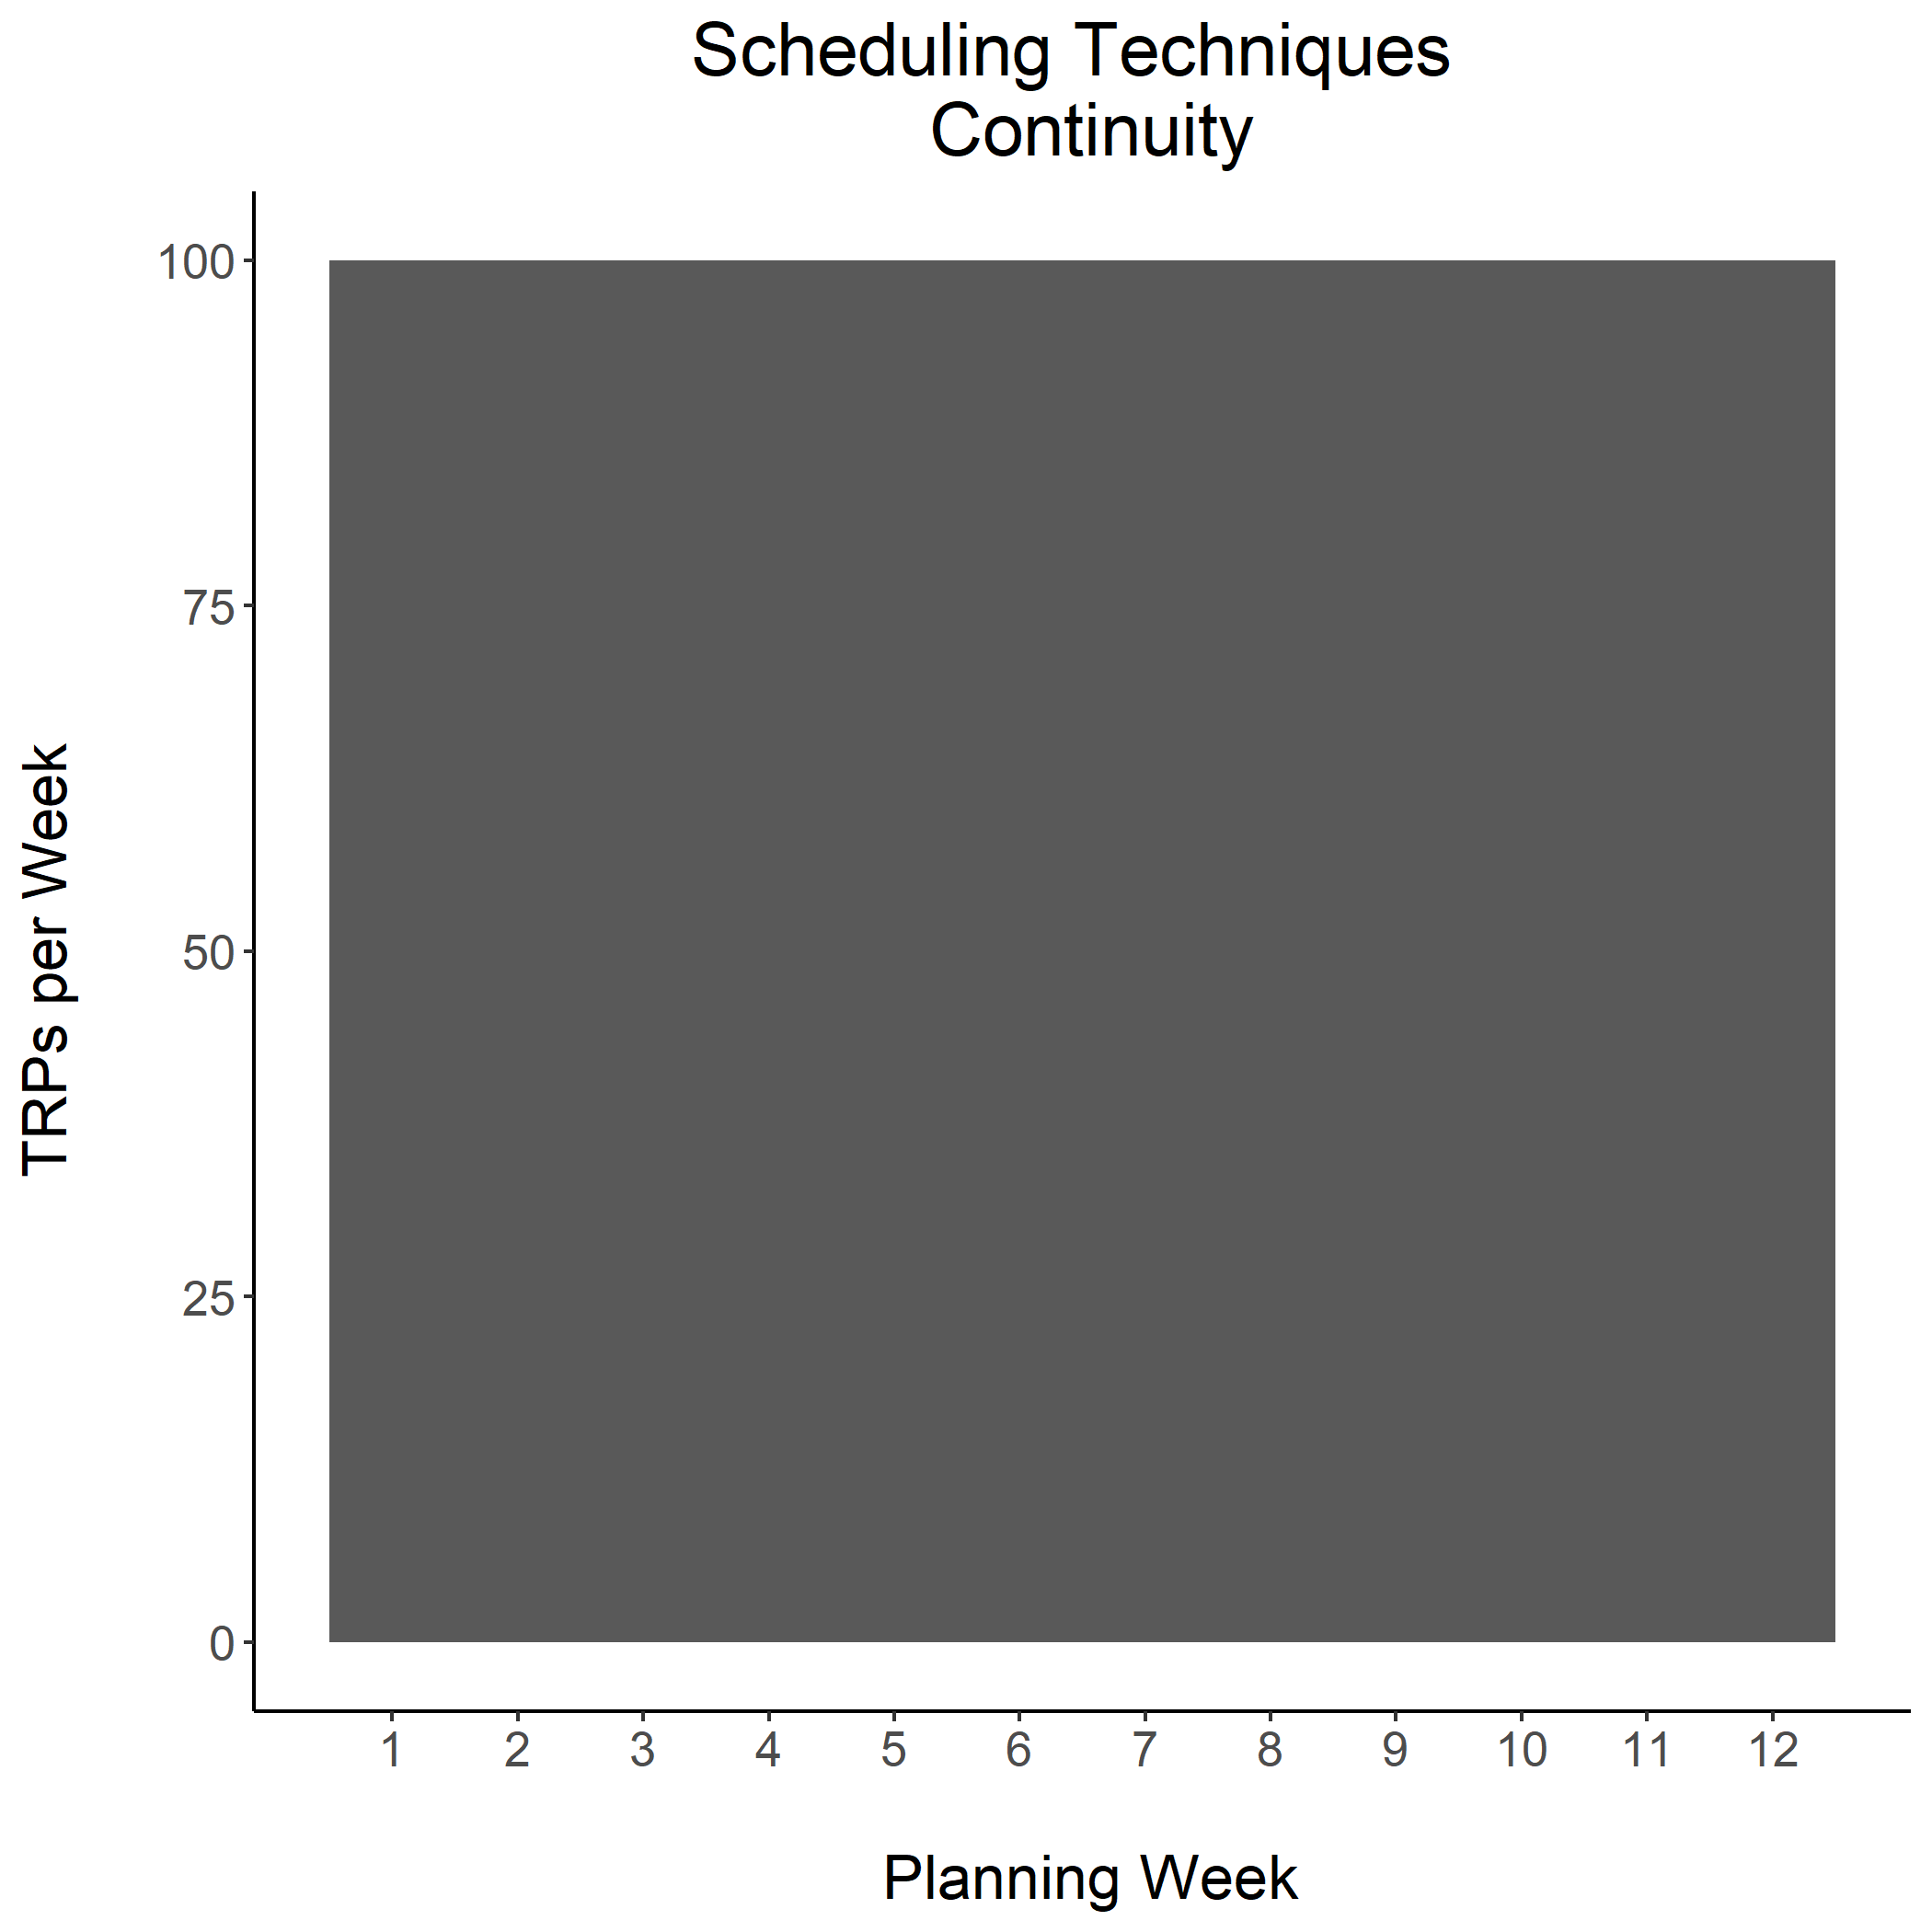
\includegraphics[height=6.8cm, trim=0.3cm 0.3cm 0.3cm 0.3cm width=6.8cm]{../BUSA_603_Ad_Response/Output/m5_0_b.png}
  \caption{Figure {\color{franklinblue} 4}: Continuity}
\end{figure}
\end{frame}

\begin{frame}[t]{Pulsing}
\begin{figure}[htbp]
  \captionsetup{justification=centering}
  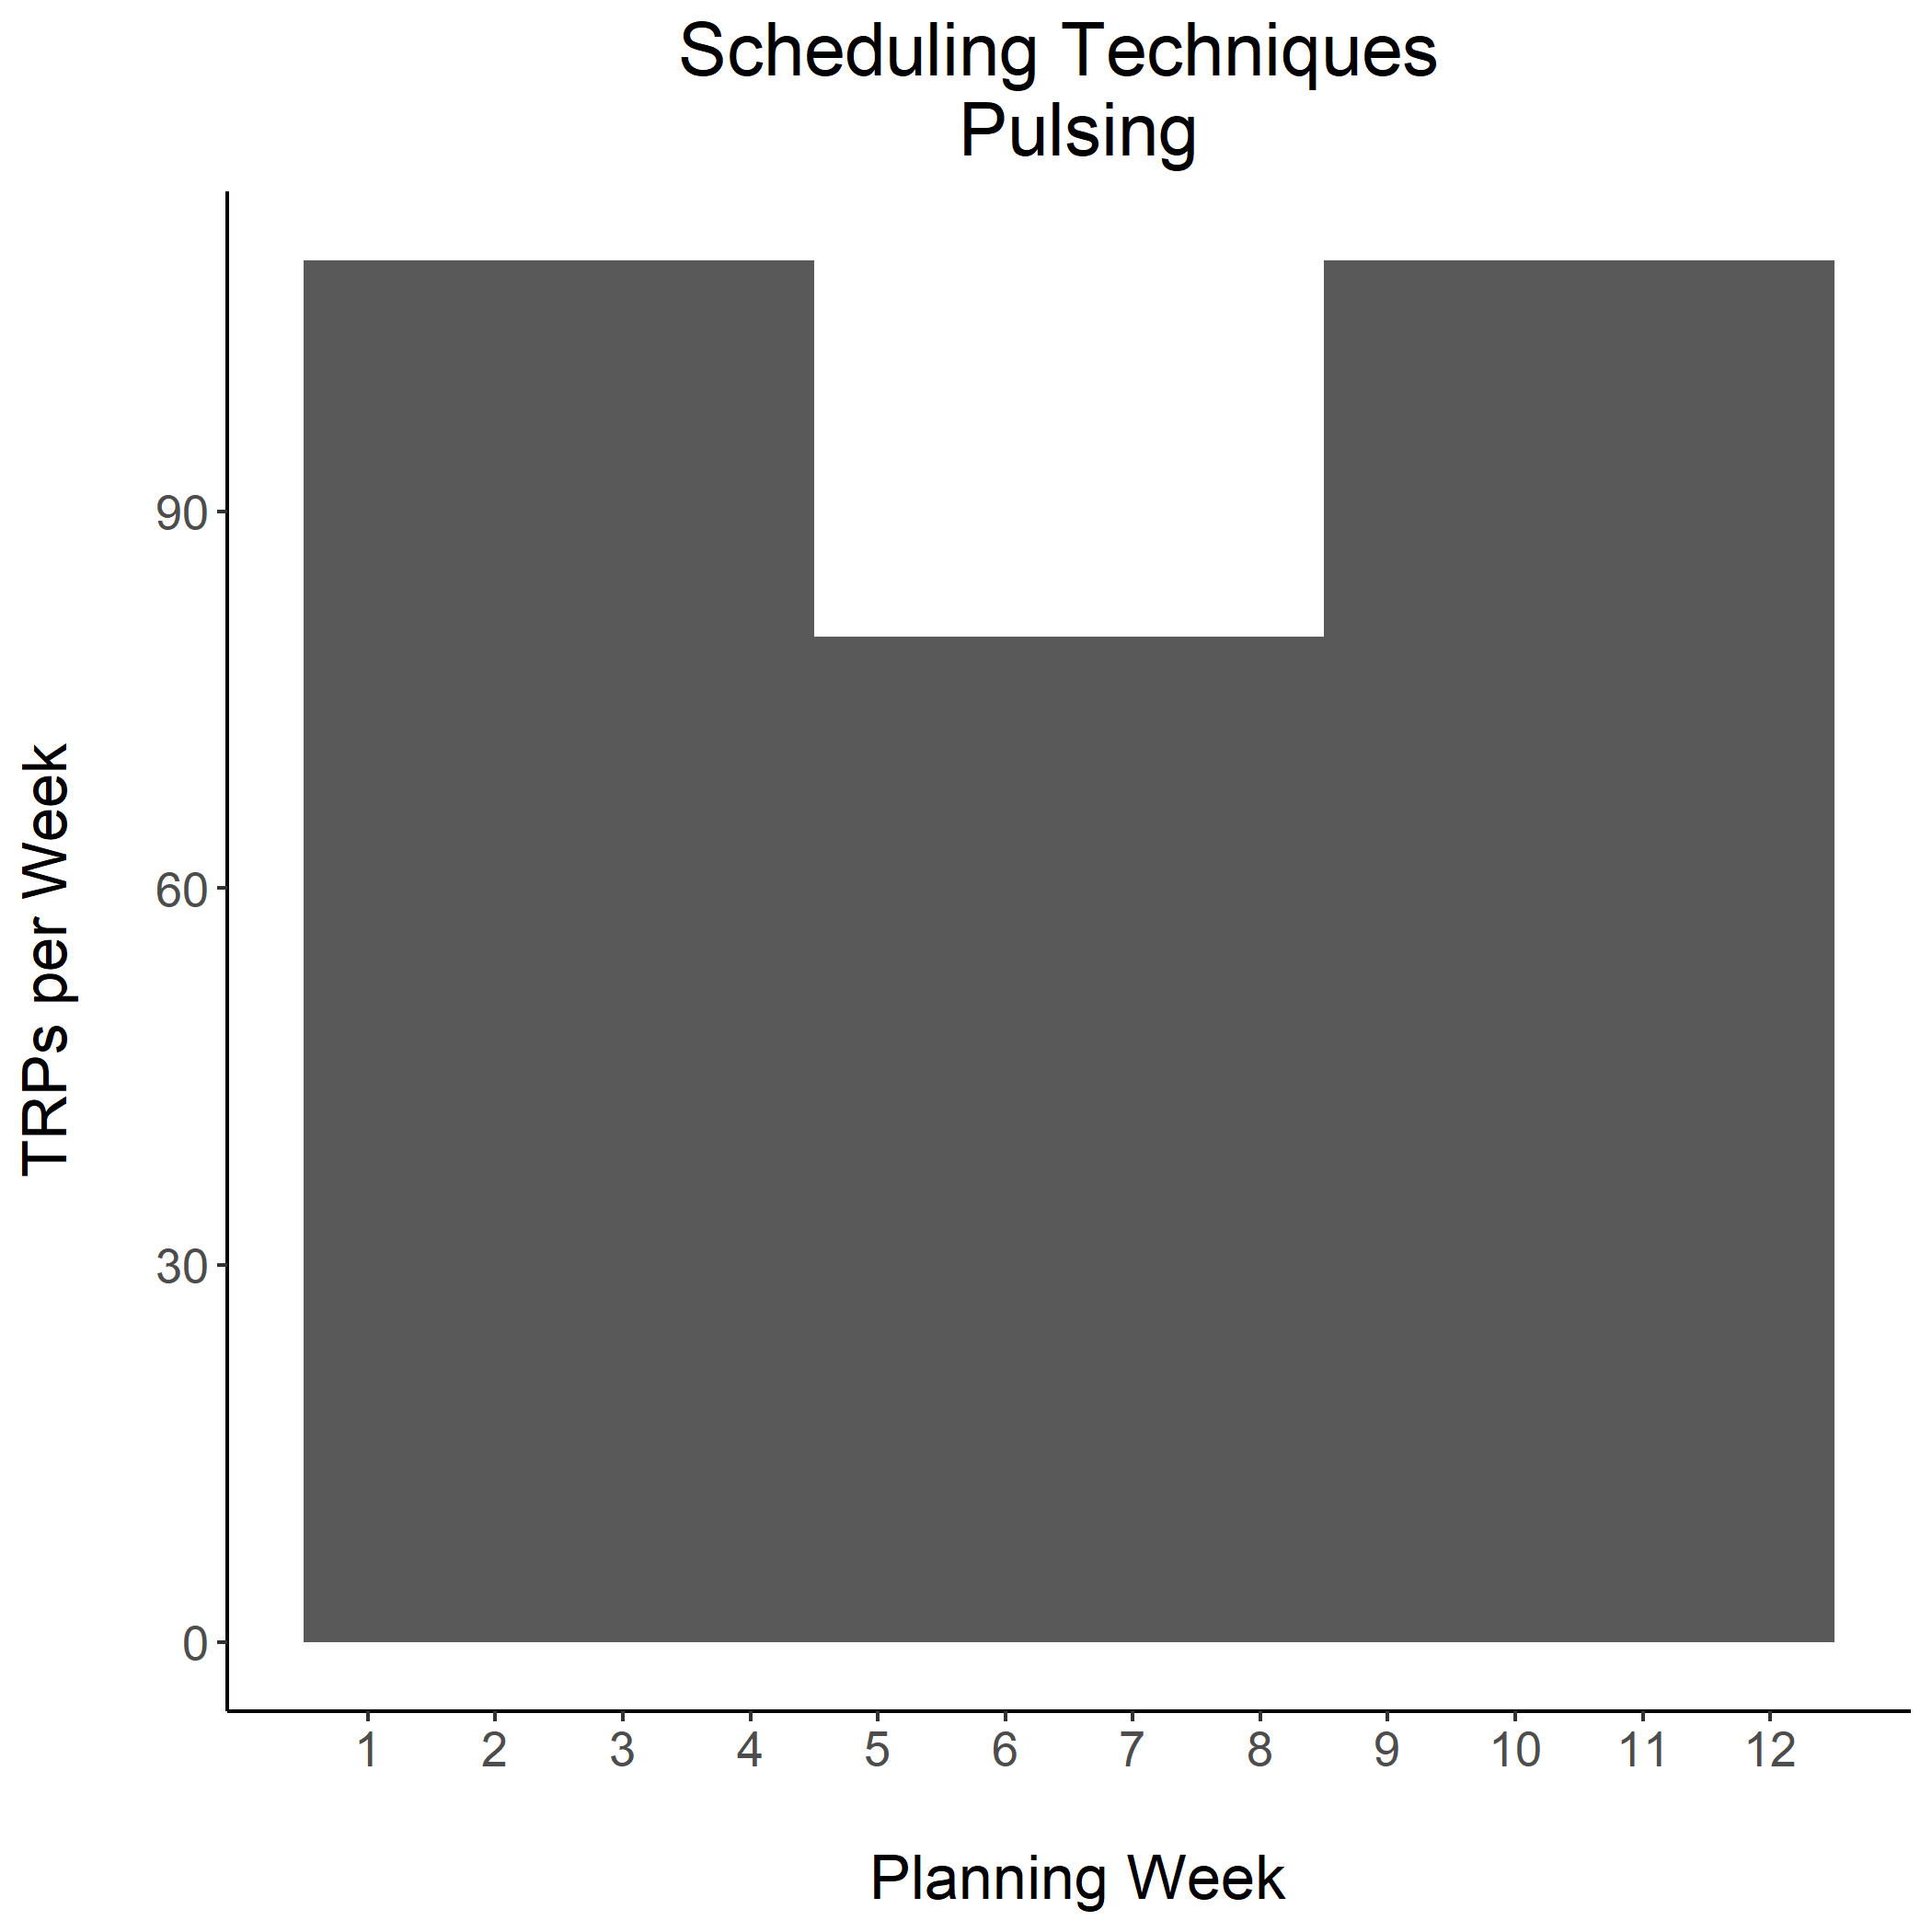
\includegraphics[height=6.8cm, trim=0.3cm 0.3cm 0.3cm 0.3cm width=6.8cm]{../BUSA_603_Ad_Response/Output/m5_0_c.png}
  \caption{Figure {\color{franklinblue} 5}: Pulsing}
\end{figure}
\end{frame}

\begin{frame}[t]{Impressions and Rating}
For \empr{measured media} -- broadcast network TV, cable network TV,  Spanish-language broadcast network TV, Spanish-language cable TV, network radio, local radio, magazines, newspapers, out-of-home and select digital advertising -- advertising planning considers expenditures, target impressions, and target rating points.\\
\vspace{1.5ex}
\begin{itemize}
  \item \empr{Target audience}, or just \underline{audience}, is a group of people defined based on their common characteristics, such as demographics and behaviors.
  \item \empr{Impressions} are the sum of all exposures.
  \item \empr{Rating} is the percentage of individuals (or homes) exposed to a particular media's program.
\end{itemize}
\end{frame}

\begin{frame}[t]{TRPs and GRPs}
\begin{itemize}
  \item \empr{Target rating points} (TRPs) are the sum of audience ratings delivered by a given list of media vehicles.  For a given audience, it is equal to 100 multiplied by audience reach multiplied by audience average frequency, where \empr{reach} is the number of different of individuals (or homes) exposed to a media schedule within a given period of time.
  \item \empr{Gross rating points} (GRPs) are the sum of ratings delivered by a given list of media vehicles.  The reference to GRPs commonly indicates \underline{household} (hh) rating points.  In contrast, TRPs are commonly refer to \underline{people} rating points.\footnote{In the advertising industry one will frequently observe and hear people interchanging TRPs and GRPs.  This is acceptable as long as the population base is being used in the reference.}  
\end{itemize}
  While GRPs are almost never used for planning, they are frequently used instead of expenditures to model the marketing mix. 
\end{frame}

\section{Patterns of Advertising Response, Wear-In, Wear-Out and Response Curves}

\begin{frame}[t]{Temporal Effects of Advertising}
There are multiple important patterns of response to advertising.  \\
\vspace{1.5ex}
\begin{figure}[htbp]
  \captionsetup{justification=centering}
  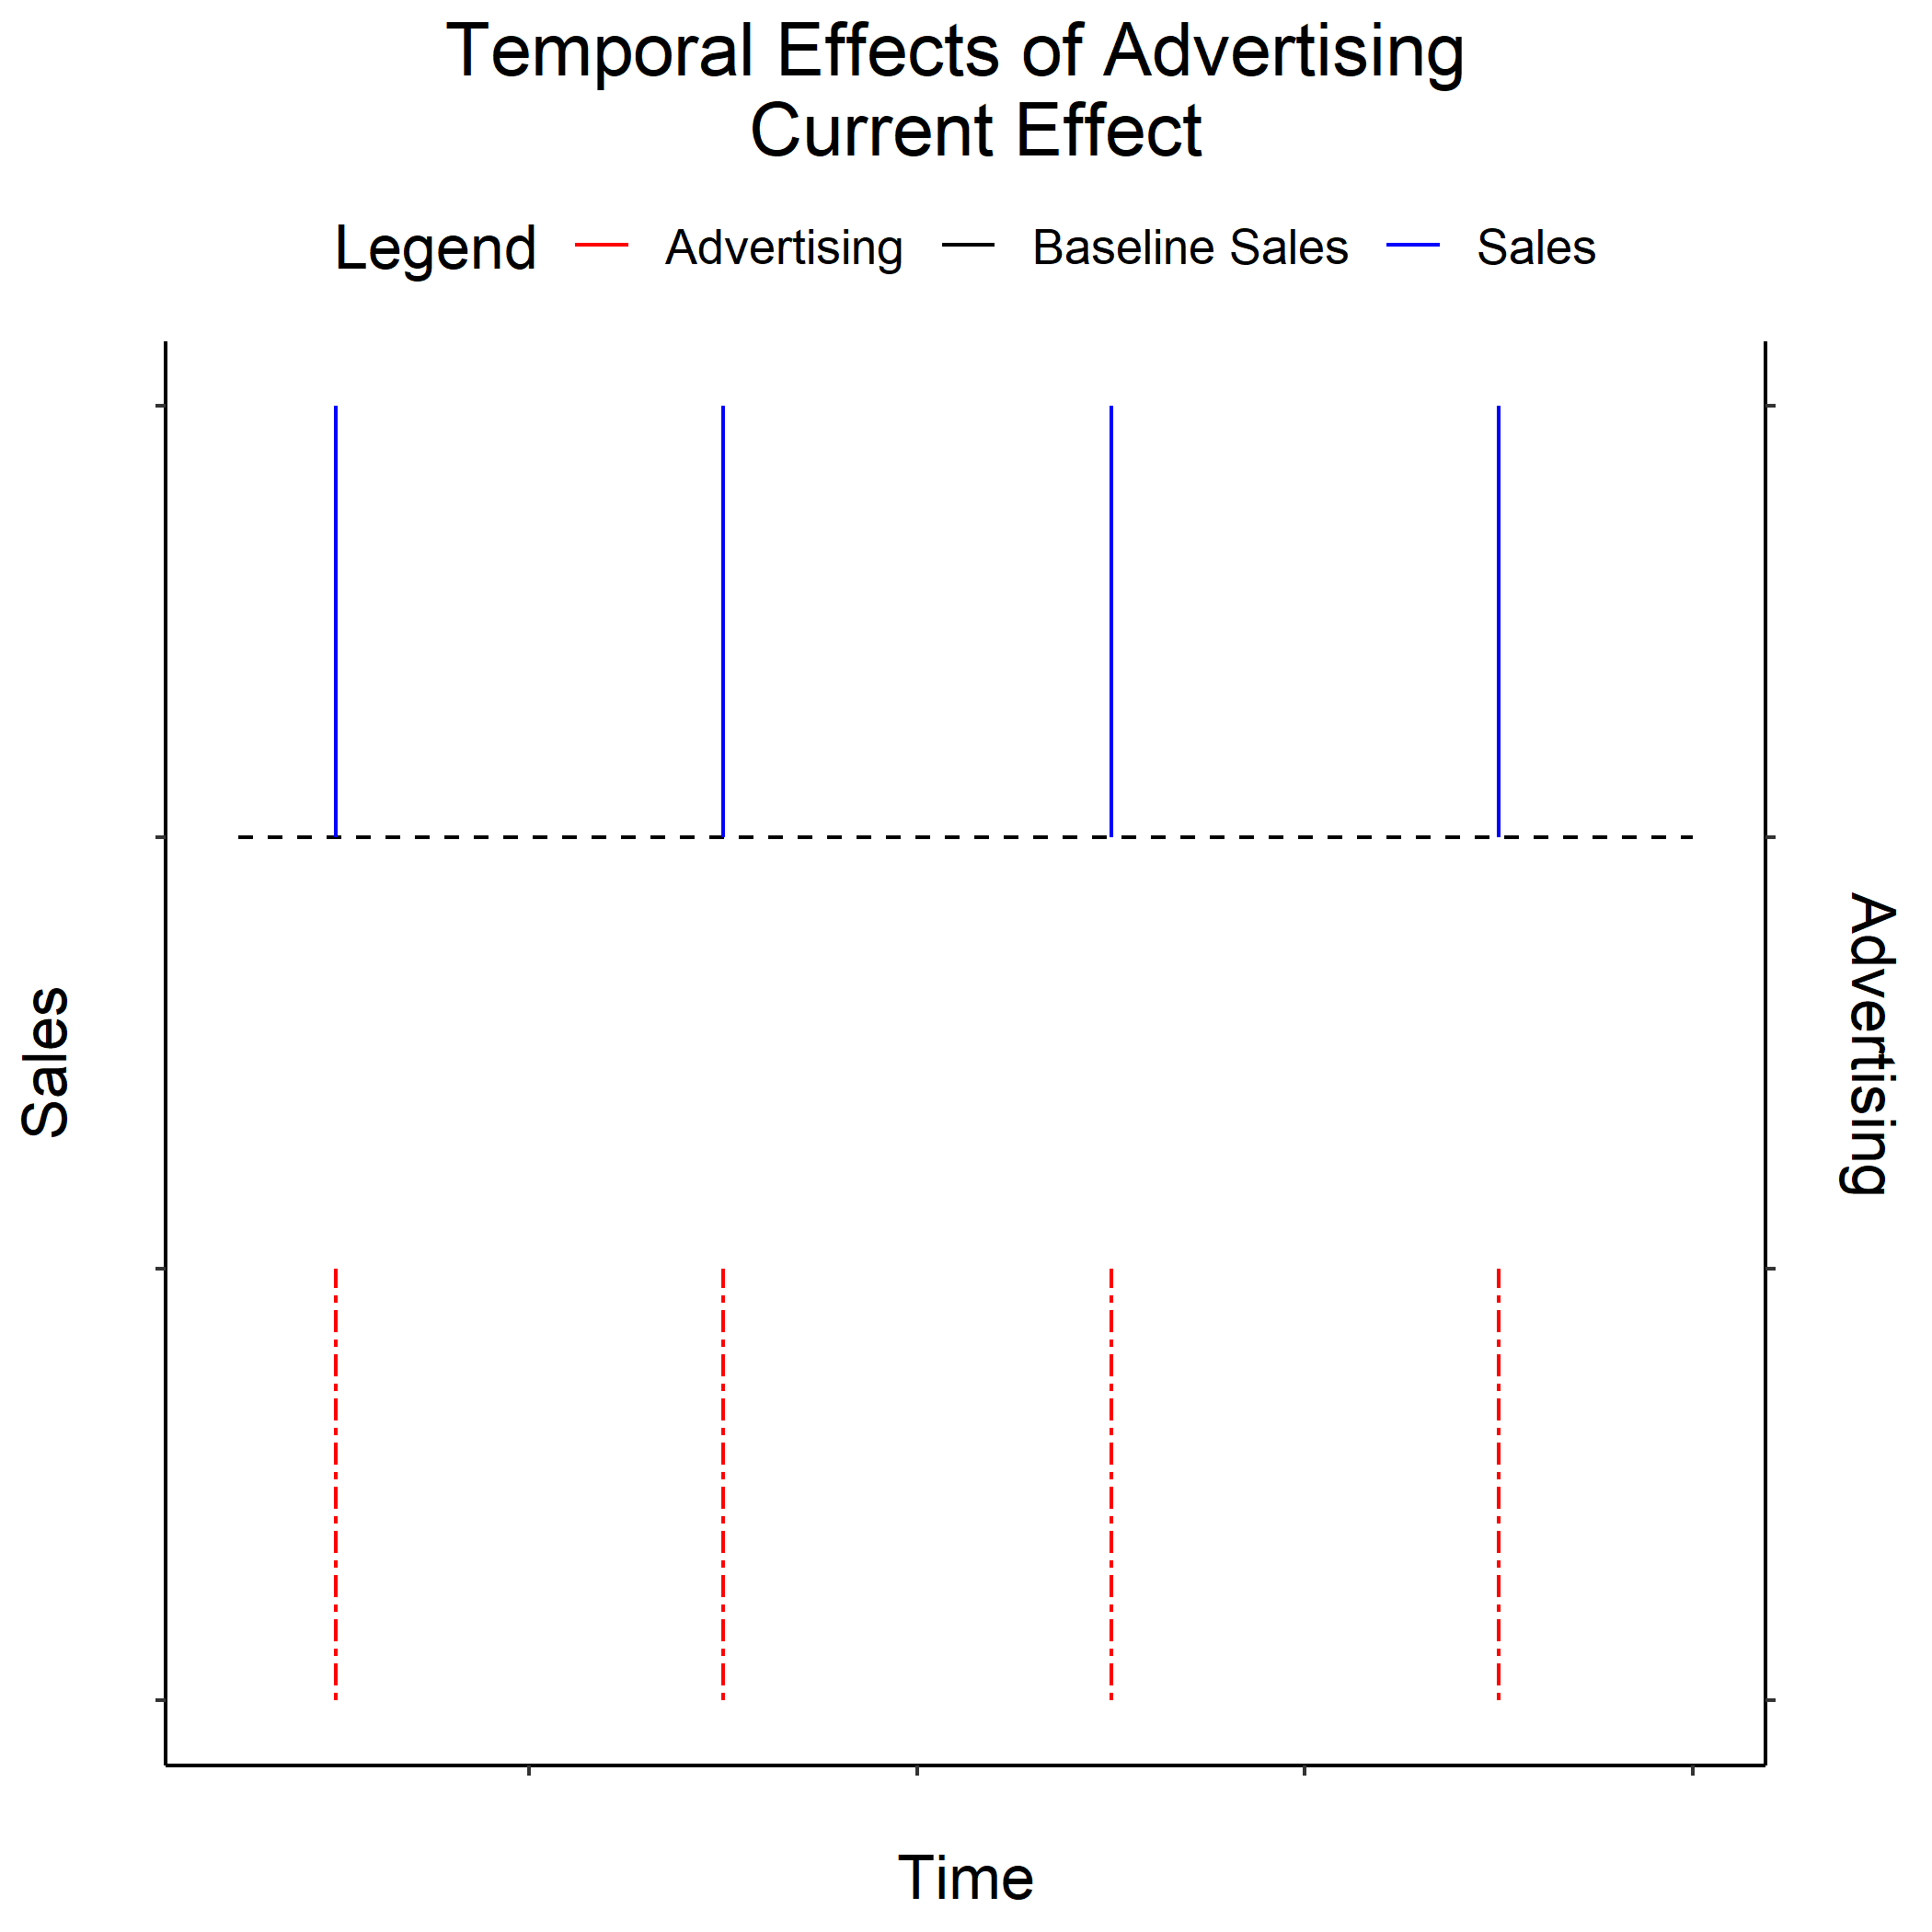
\includegraphics[height=5.8cm, trim=0.3cm 0.3cm 0.3cm 0.3cm width=5.8cm]{../BUSA_603_Ad_Response/Output/m5_1.png}
  \caption{Figure {\color{franklinblue} 6}: Current Effect}
\end{figure}
\end{frame}

\begin{frame}[t]{Carryover Effects of Short Duration}
\begin{figure}[htbp]
  \captionsetup{justification=centering}
  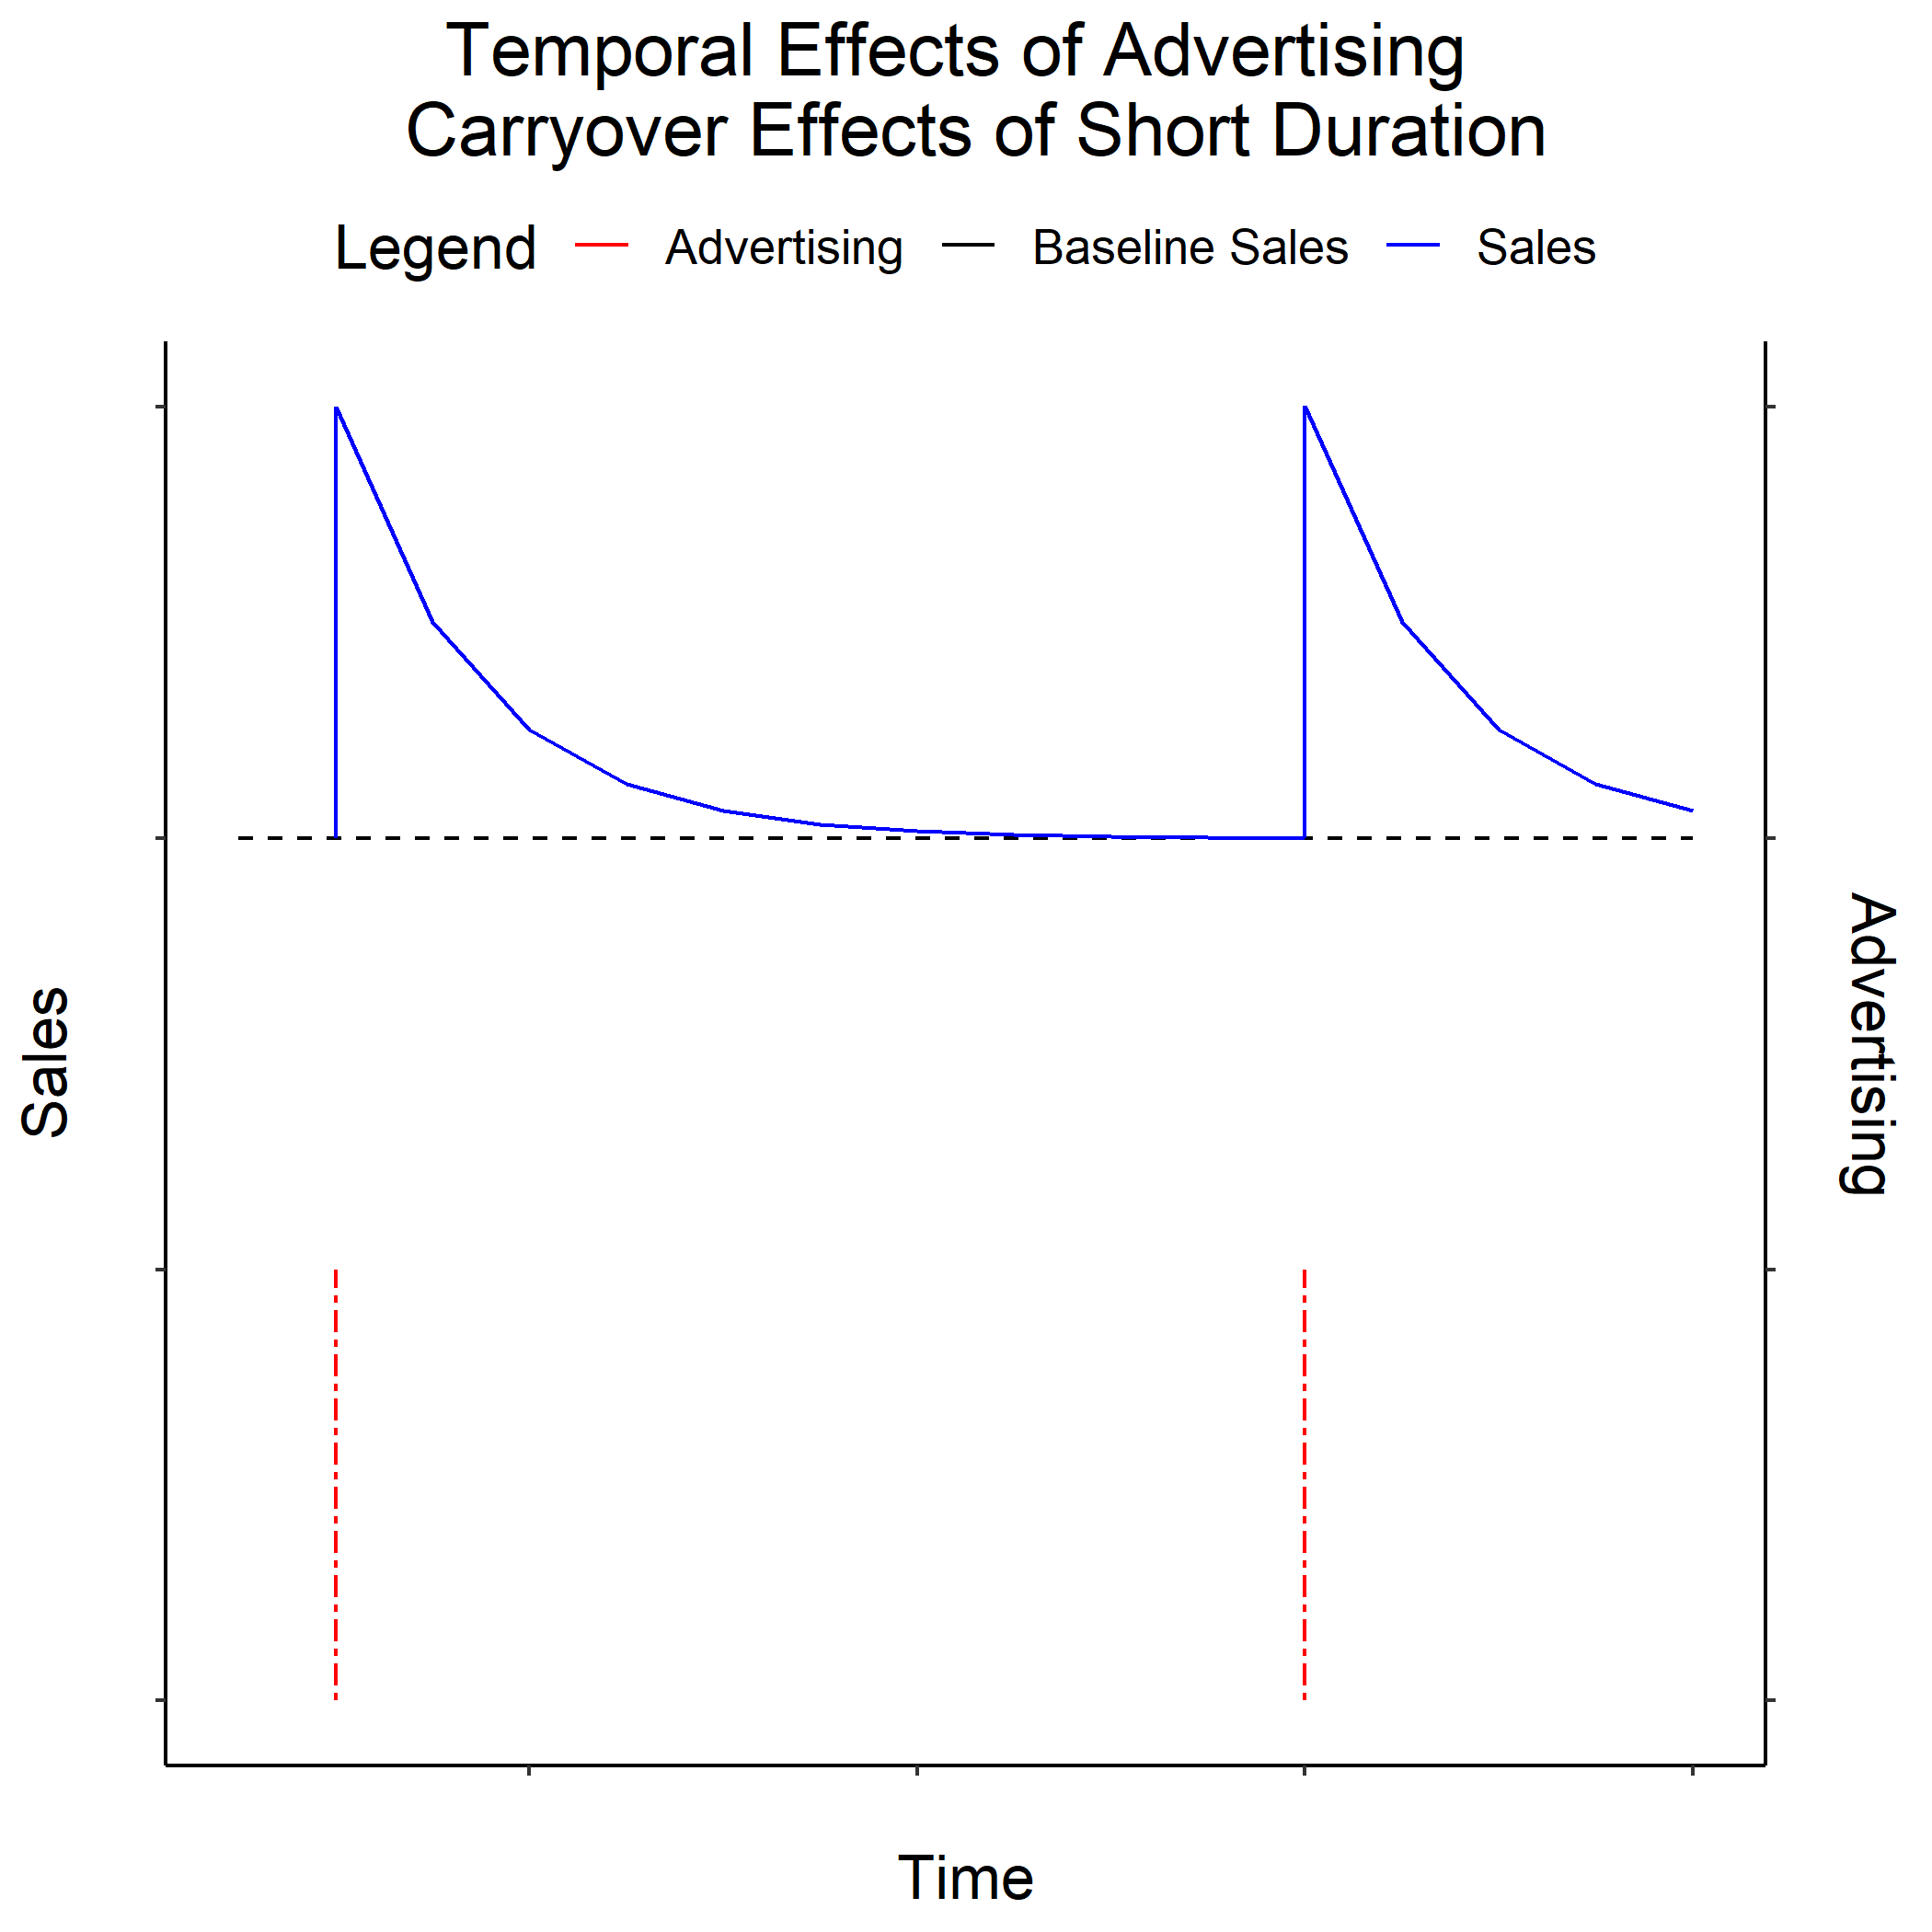
\includegraphics[height=6.8cm, trim=0.3cm 0.3cm 0.3cm 0.3cm width=6.8cm]{../BUSA_603_Ad_Response/Output/m5_2.png}
  \caption{Figure {\color{franklinblue} 7}: Carryover Effects of Short Duration}
\end{figure}
\end{frame}

\begin{frame}[t]{Carryover Effects of Long Duration}
\begin{figure}[htbp]
  \captionsetup{justification=centering}
  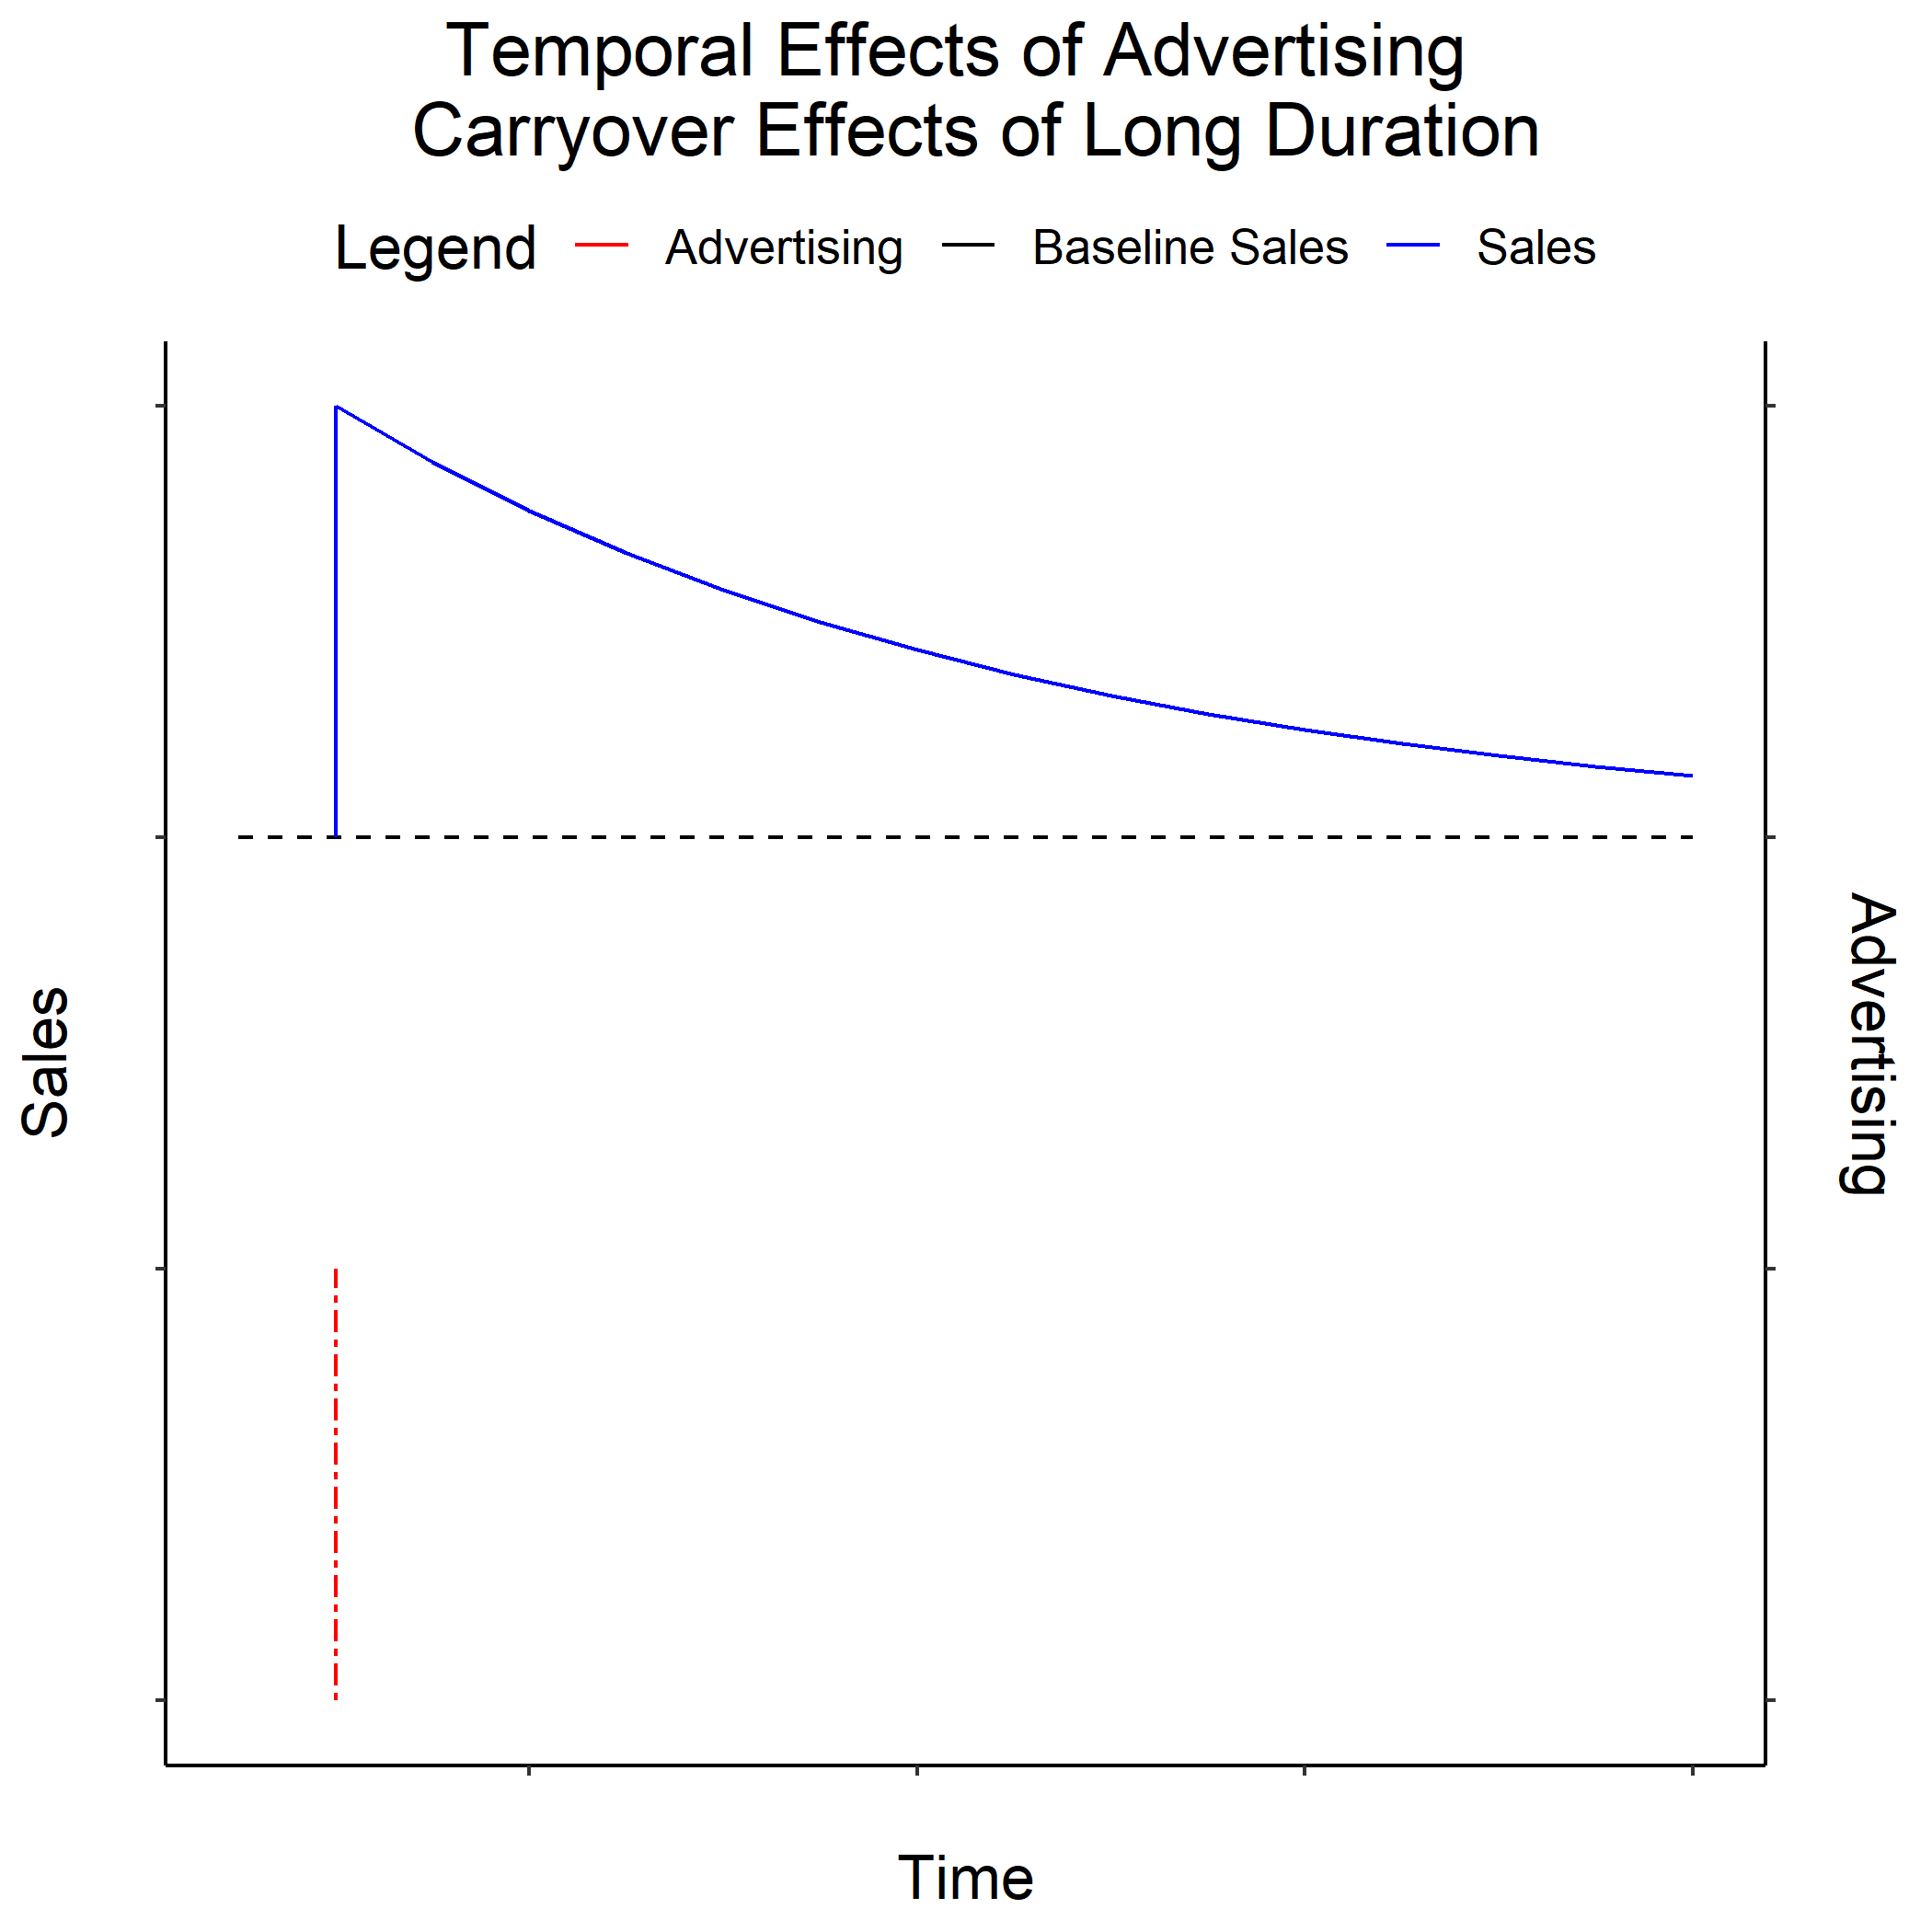
\includegraphics[height=6.8cm, trim=0.3cm 0.3cm 0.3cm 0.3cm width=6.8cm]{../BUSA_603_Ad_Response/Output/m5_3.png}
  \caption{Figure {\color{franklinblue} 8}: Carryover Effects of Long Duration}
\end{figure}
\end{frame}

\begin{frame}[t]{Persistent Effect}
\begin{figure}[htbp]
  \captionsetup{justification=centering}
  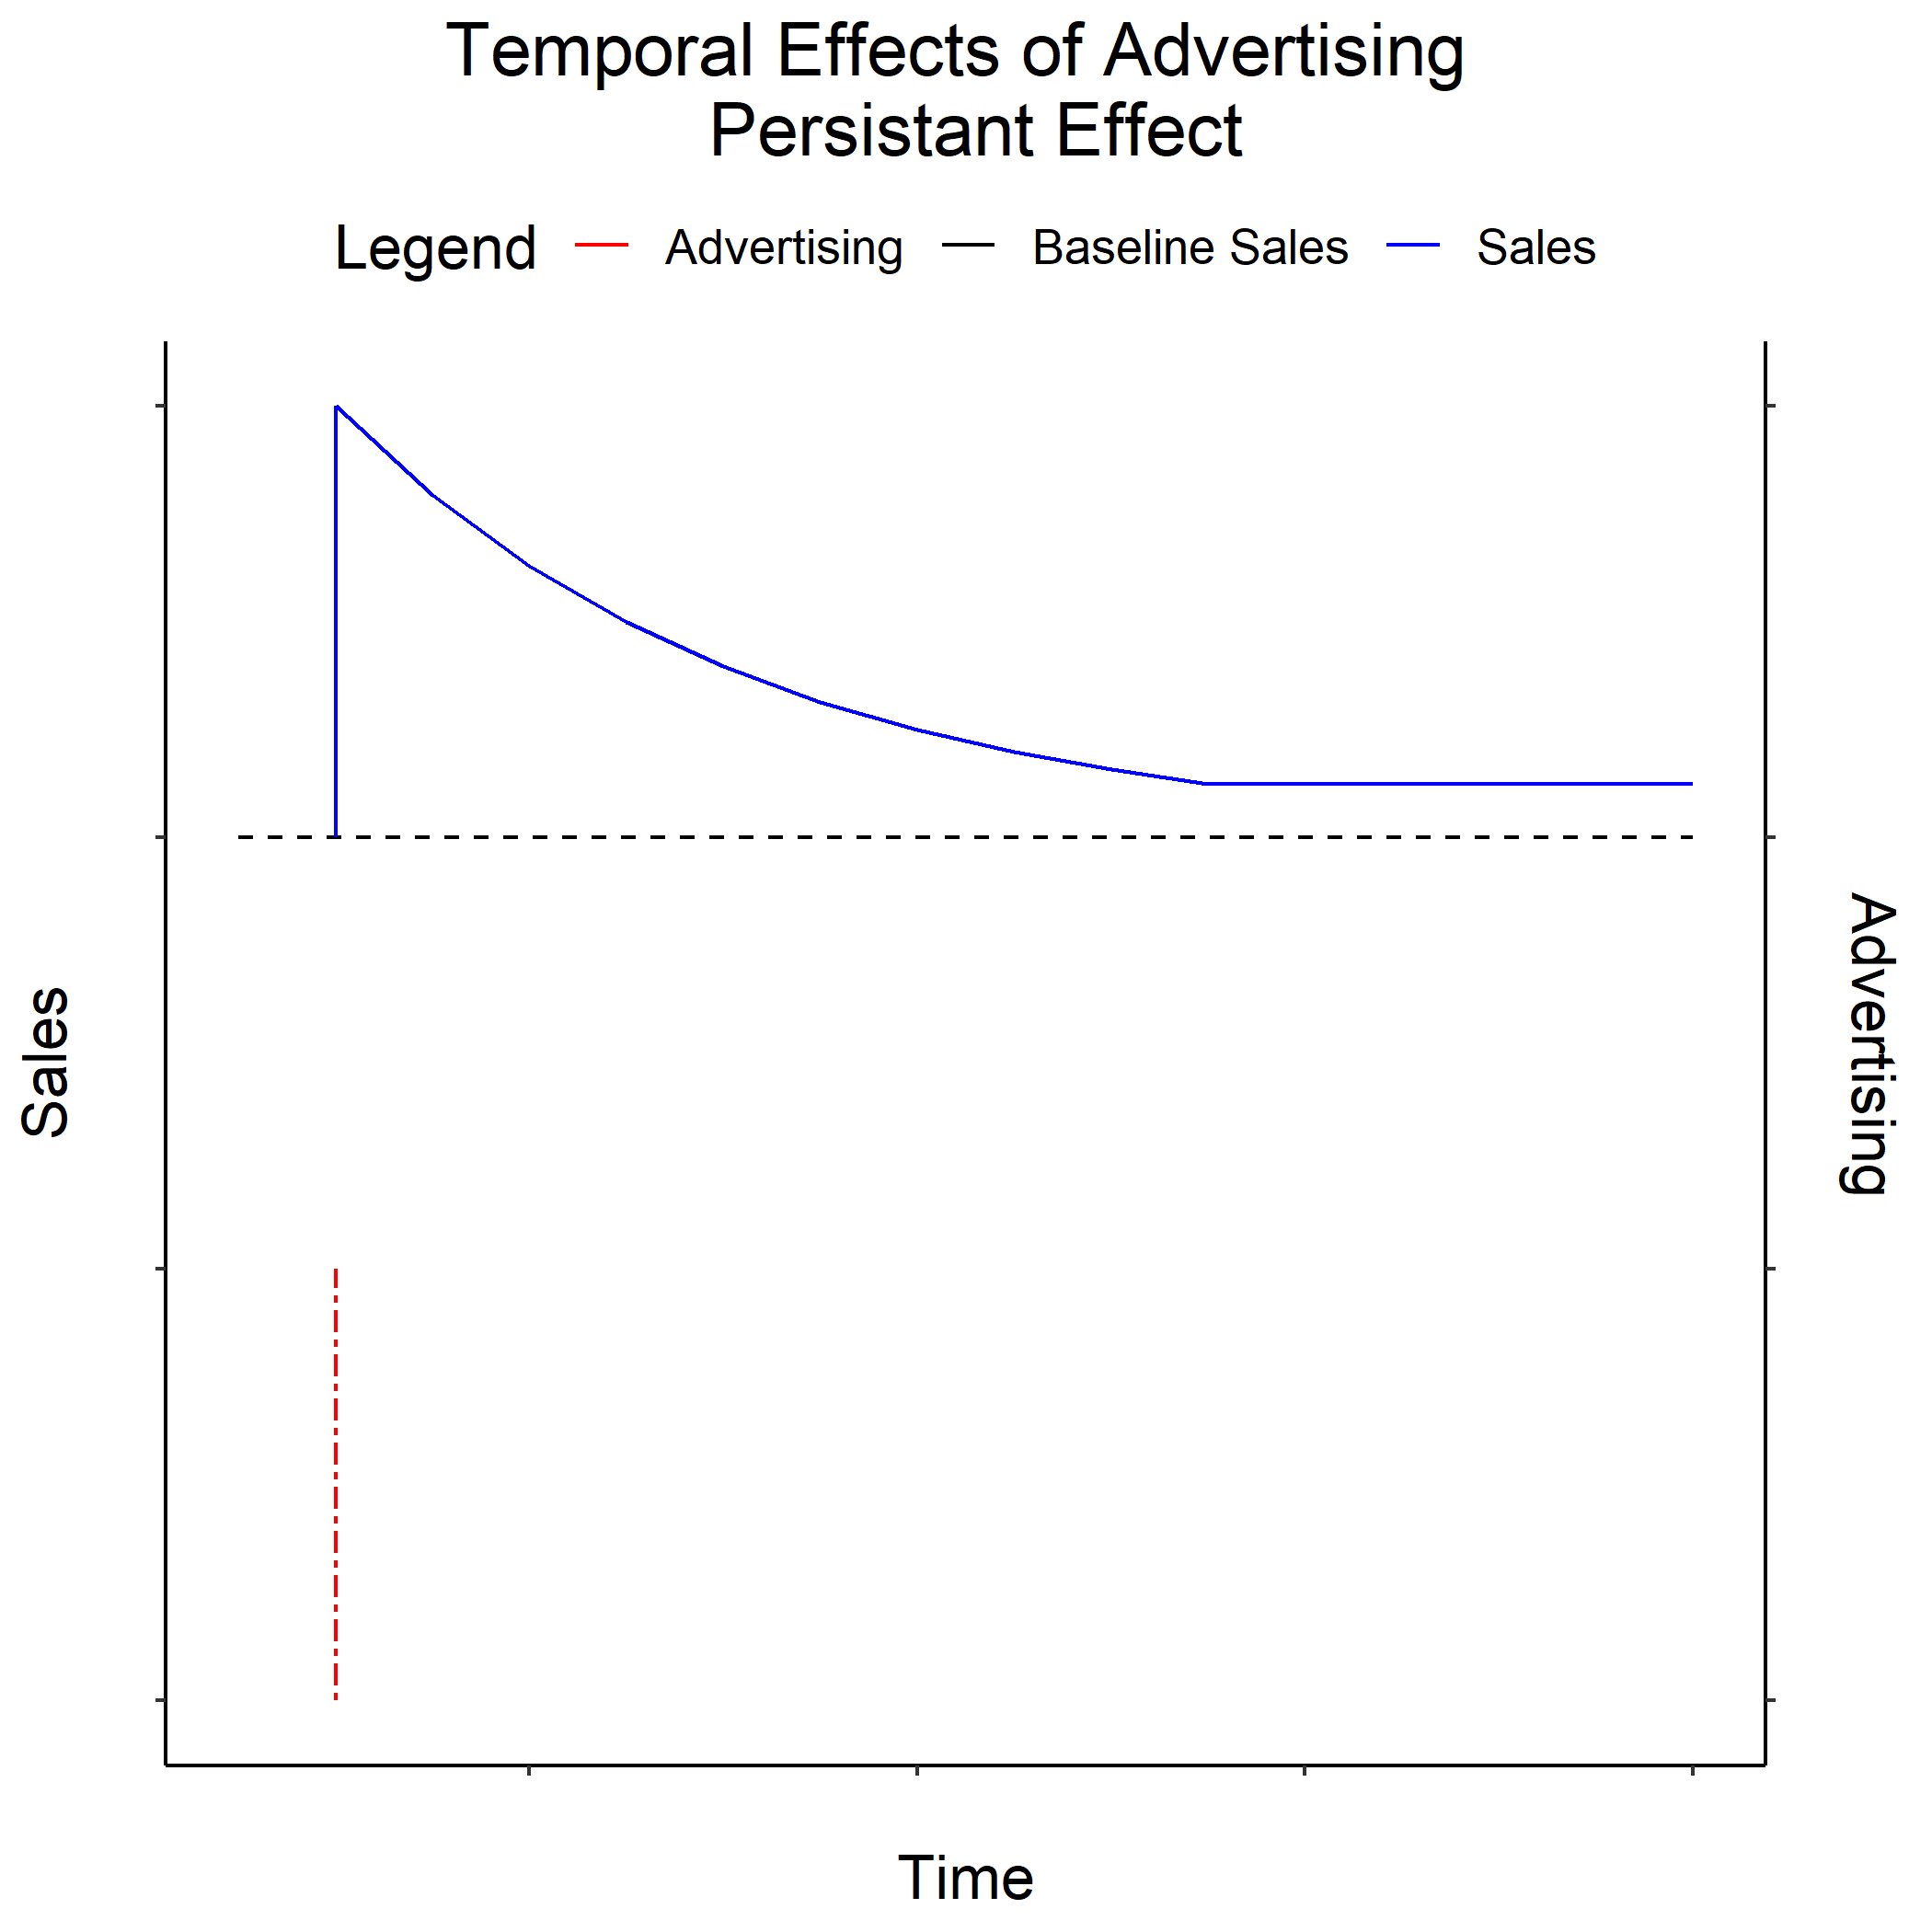
\includegraphics[height=6.8cm, trim=0.3cm 0.3cm 0.3cm 0.3cm width=6.8cm]{../BUSA_603_Ad_Response/Output/m5_4.png}
  \caption{Figure {\color{franklinblue} 9}: Persistent Effect}
\end{figure}
\end{frame}

\begin{frame}[t]{Adstock}
A simple exponential function specification, referred to as \empr{adstock}, leads to many of the effects given above.\footnote{The idea of adstock originated from \cite{broadbent1979}.} \\
\vspace{-0.5ex}
\begin{equation}
 \text{Adstock}_t = \text{GRPs}_t + \phi \text{Adstock}_{t-1},
\end{equation}
where $\phi = 0.5^{1/\varphi}$.  $\phi$ is referred to as the \empr{retention rate}, and $\varphi$ is the \empr{half-life}. \\
\vspace{1.5ex}
A ``two-week half-life'' means that it takes two weeks for the awareness of advertising to decay to half its present level. \\
\vspace{1.5ex}
Beyond its use as an input to an adstock explanatory variable in a model to measure advertising effectiveness,   half-life enables brand managers to  efficiently space advertising schedules to maximize the effect of each advertising exposure.
\end{frame}

\begin{frame}[t]{Dynamic Effects}
\empr{Wear-in} is the increase in the response of sales to advertising, from one week to the next of a campaign, even though advertising occurs at the same level each week.  \\
\vspace{1.5ex}
If wear-in occurs, it typically occurs at the start of a campaign. It could occur because repetition of a campaign in subsequent periods enables more people to see the ad, talk about it,  think about it, and respond to it than would have
done so on the very first period of the campaign. \\
\vspace{1.5ex}
\empr{Wear-out} is the decline in sales response of sales to advertising from week to week of a campaign, even though advertising occurs at the same level each week. \\
\vspace{1.5ex}
Wear-out typically occurs at the end of a campaign because of consumer tedium.
\end{frame}

\begin{frame}[t]{Wear-In and Wear-Out}
\begin{figure}[htbp]
  \captionsetup{justification=centering}
  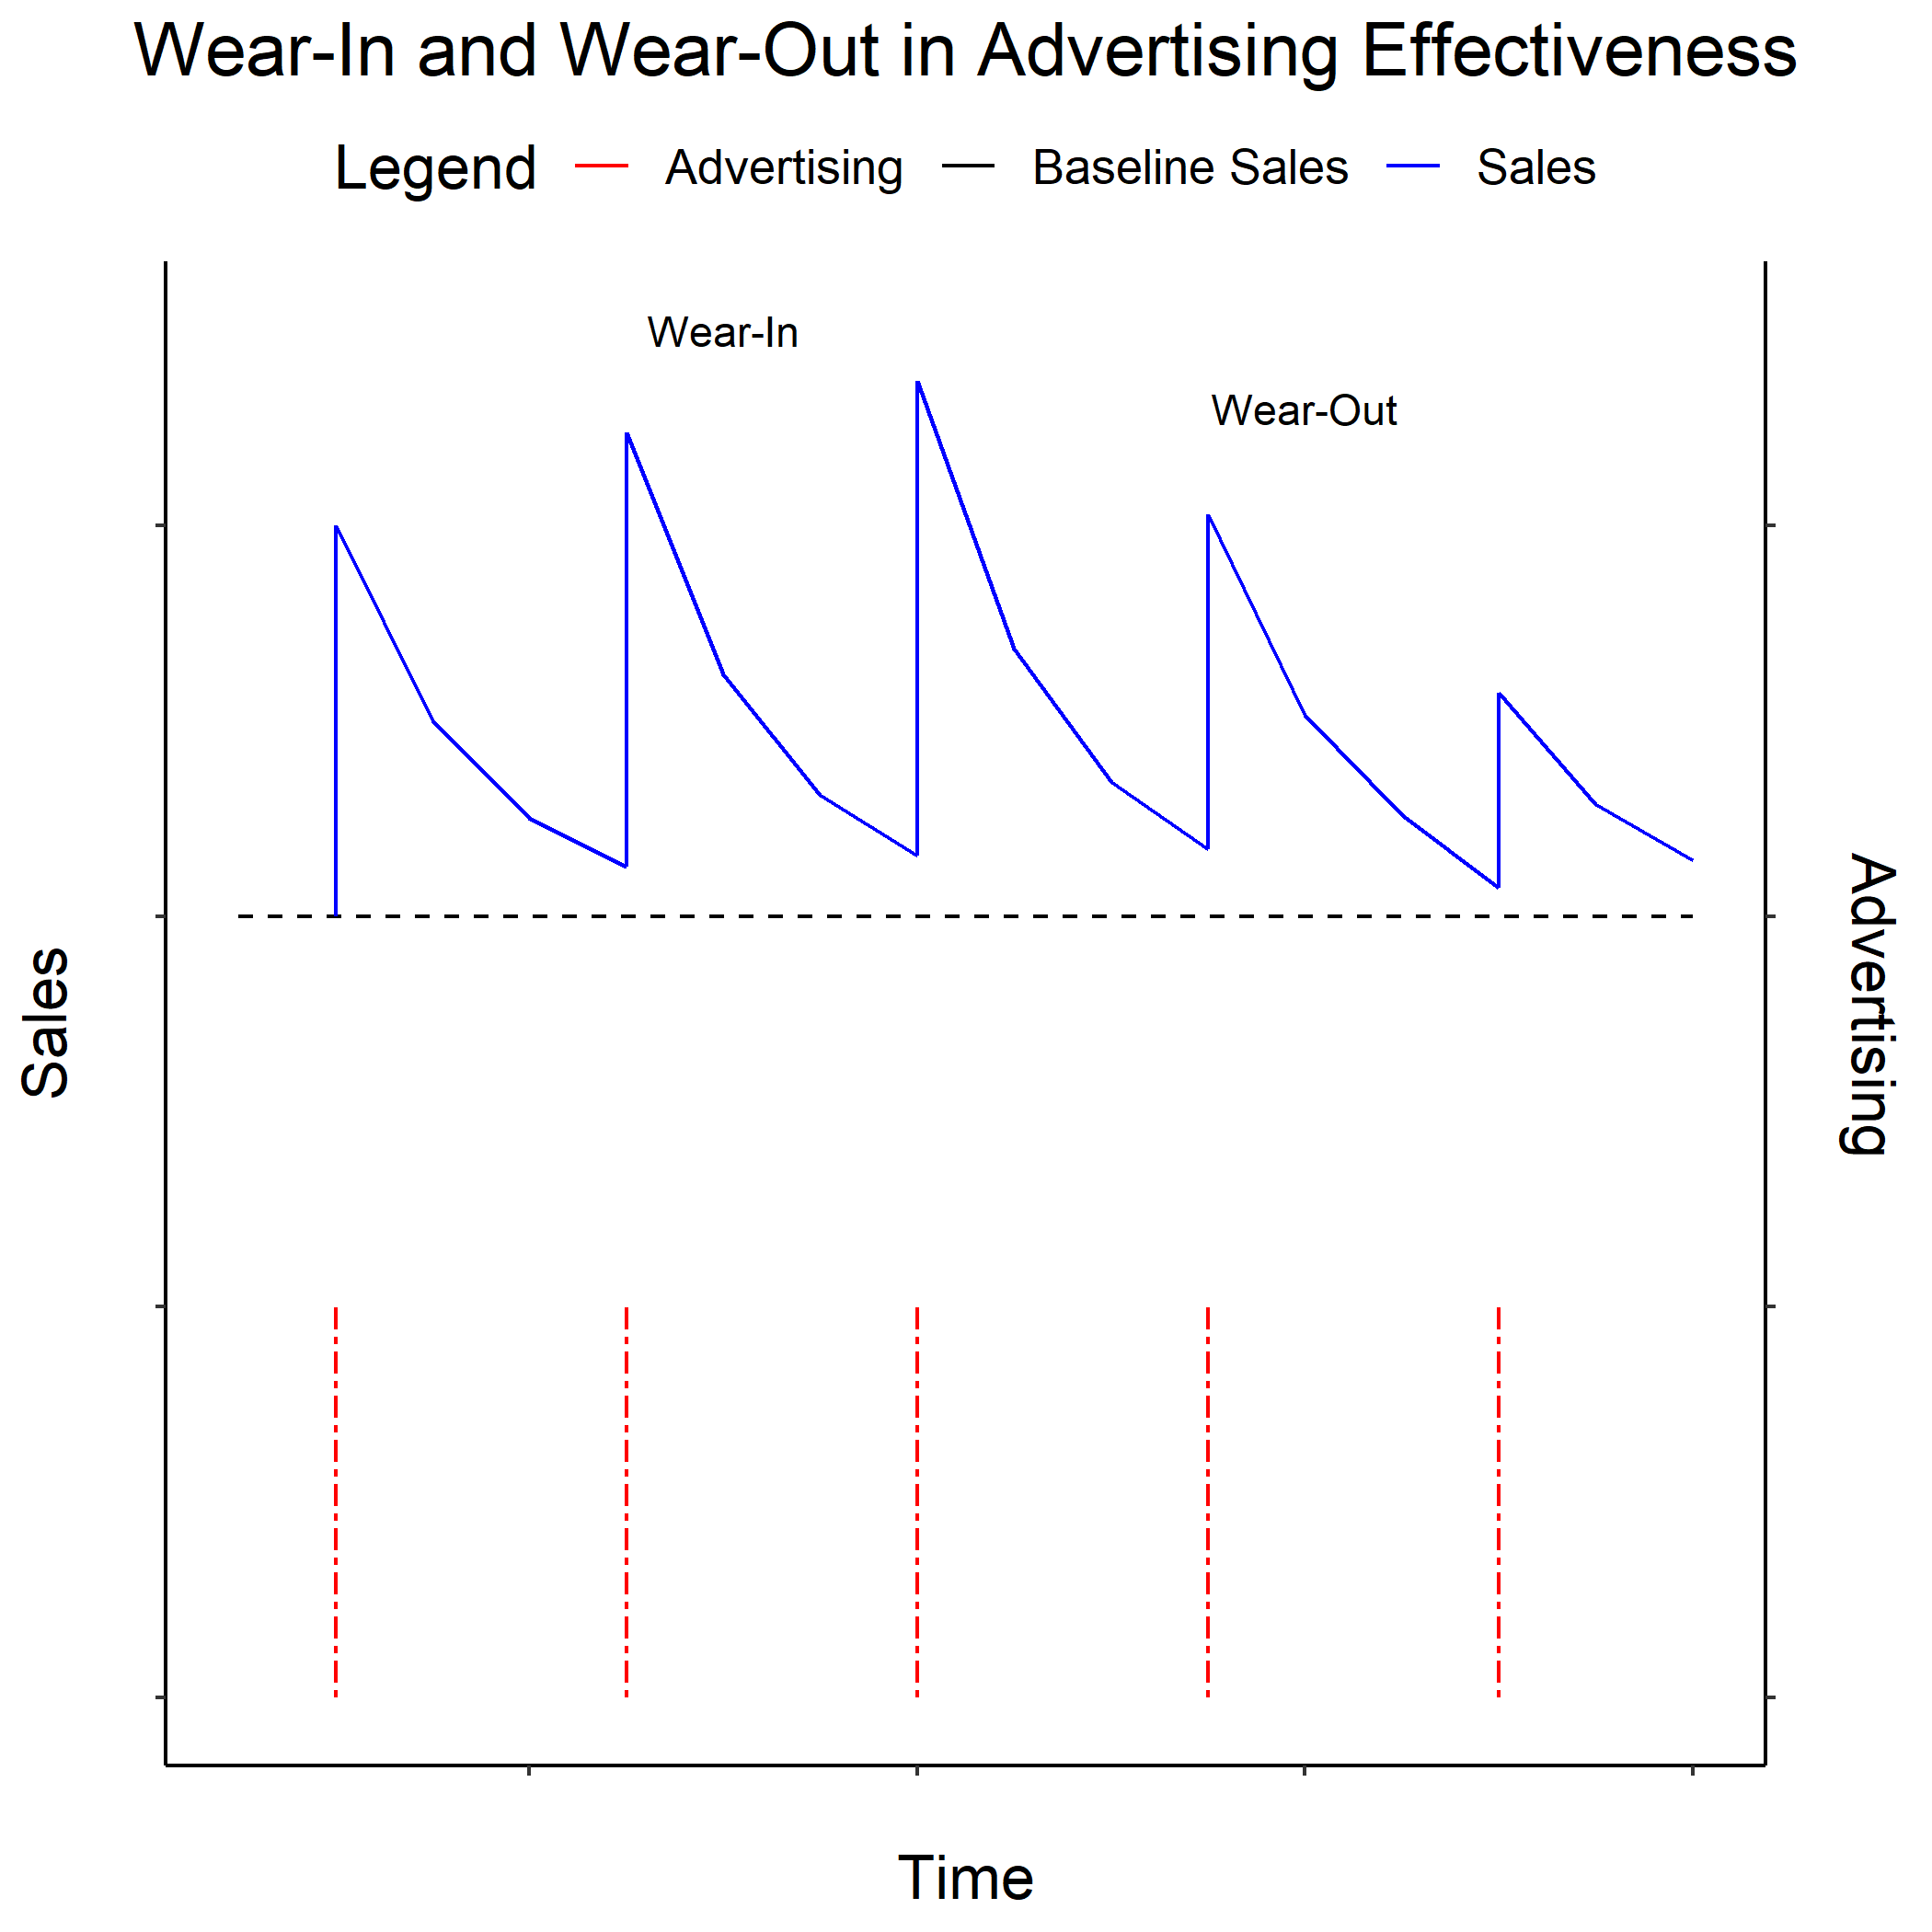
\includegraphics[height=6.8cm, trim=0.3cm 0.3cm 0.3cm 0.3cm width=6.8cm]{../BUSA_603_Ad_Response/Output/m5_5.png}
  \caption{Figure {\color{franklinblue} 10}: Wear-in and Wear-out}
\end{figure}
\end{frame}


\begin{frame}[t]{Linear and Nonlinear Response to Advertising}
\begin{figure}[htbp]
  \captionsetup{justification=centering}
  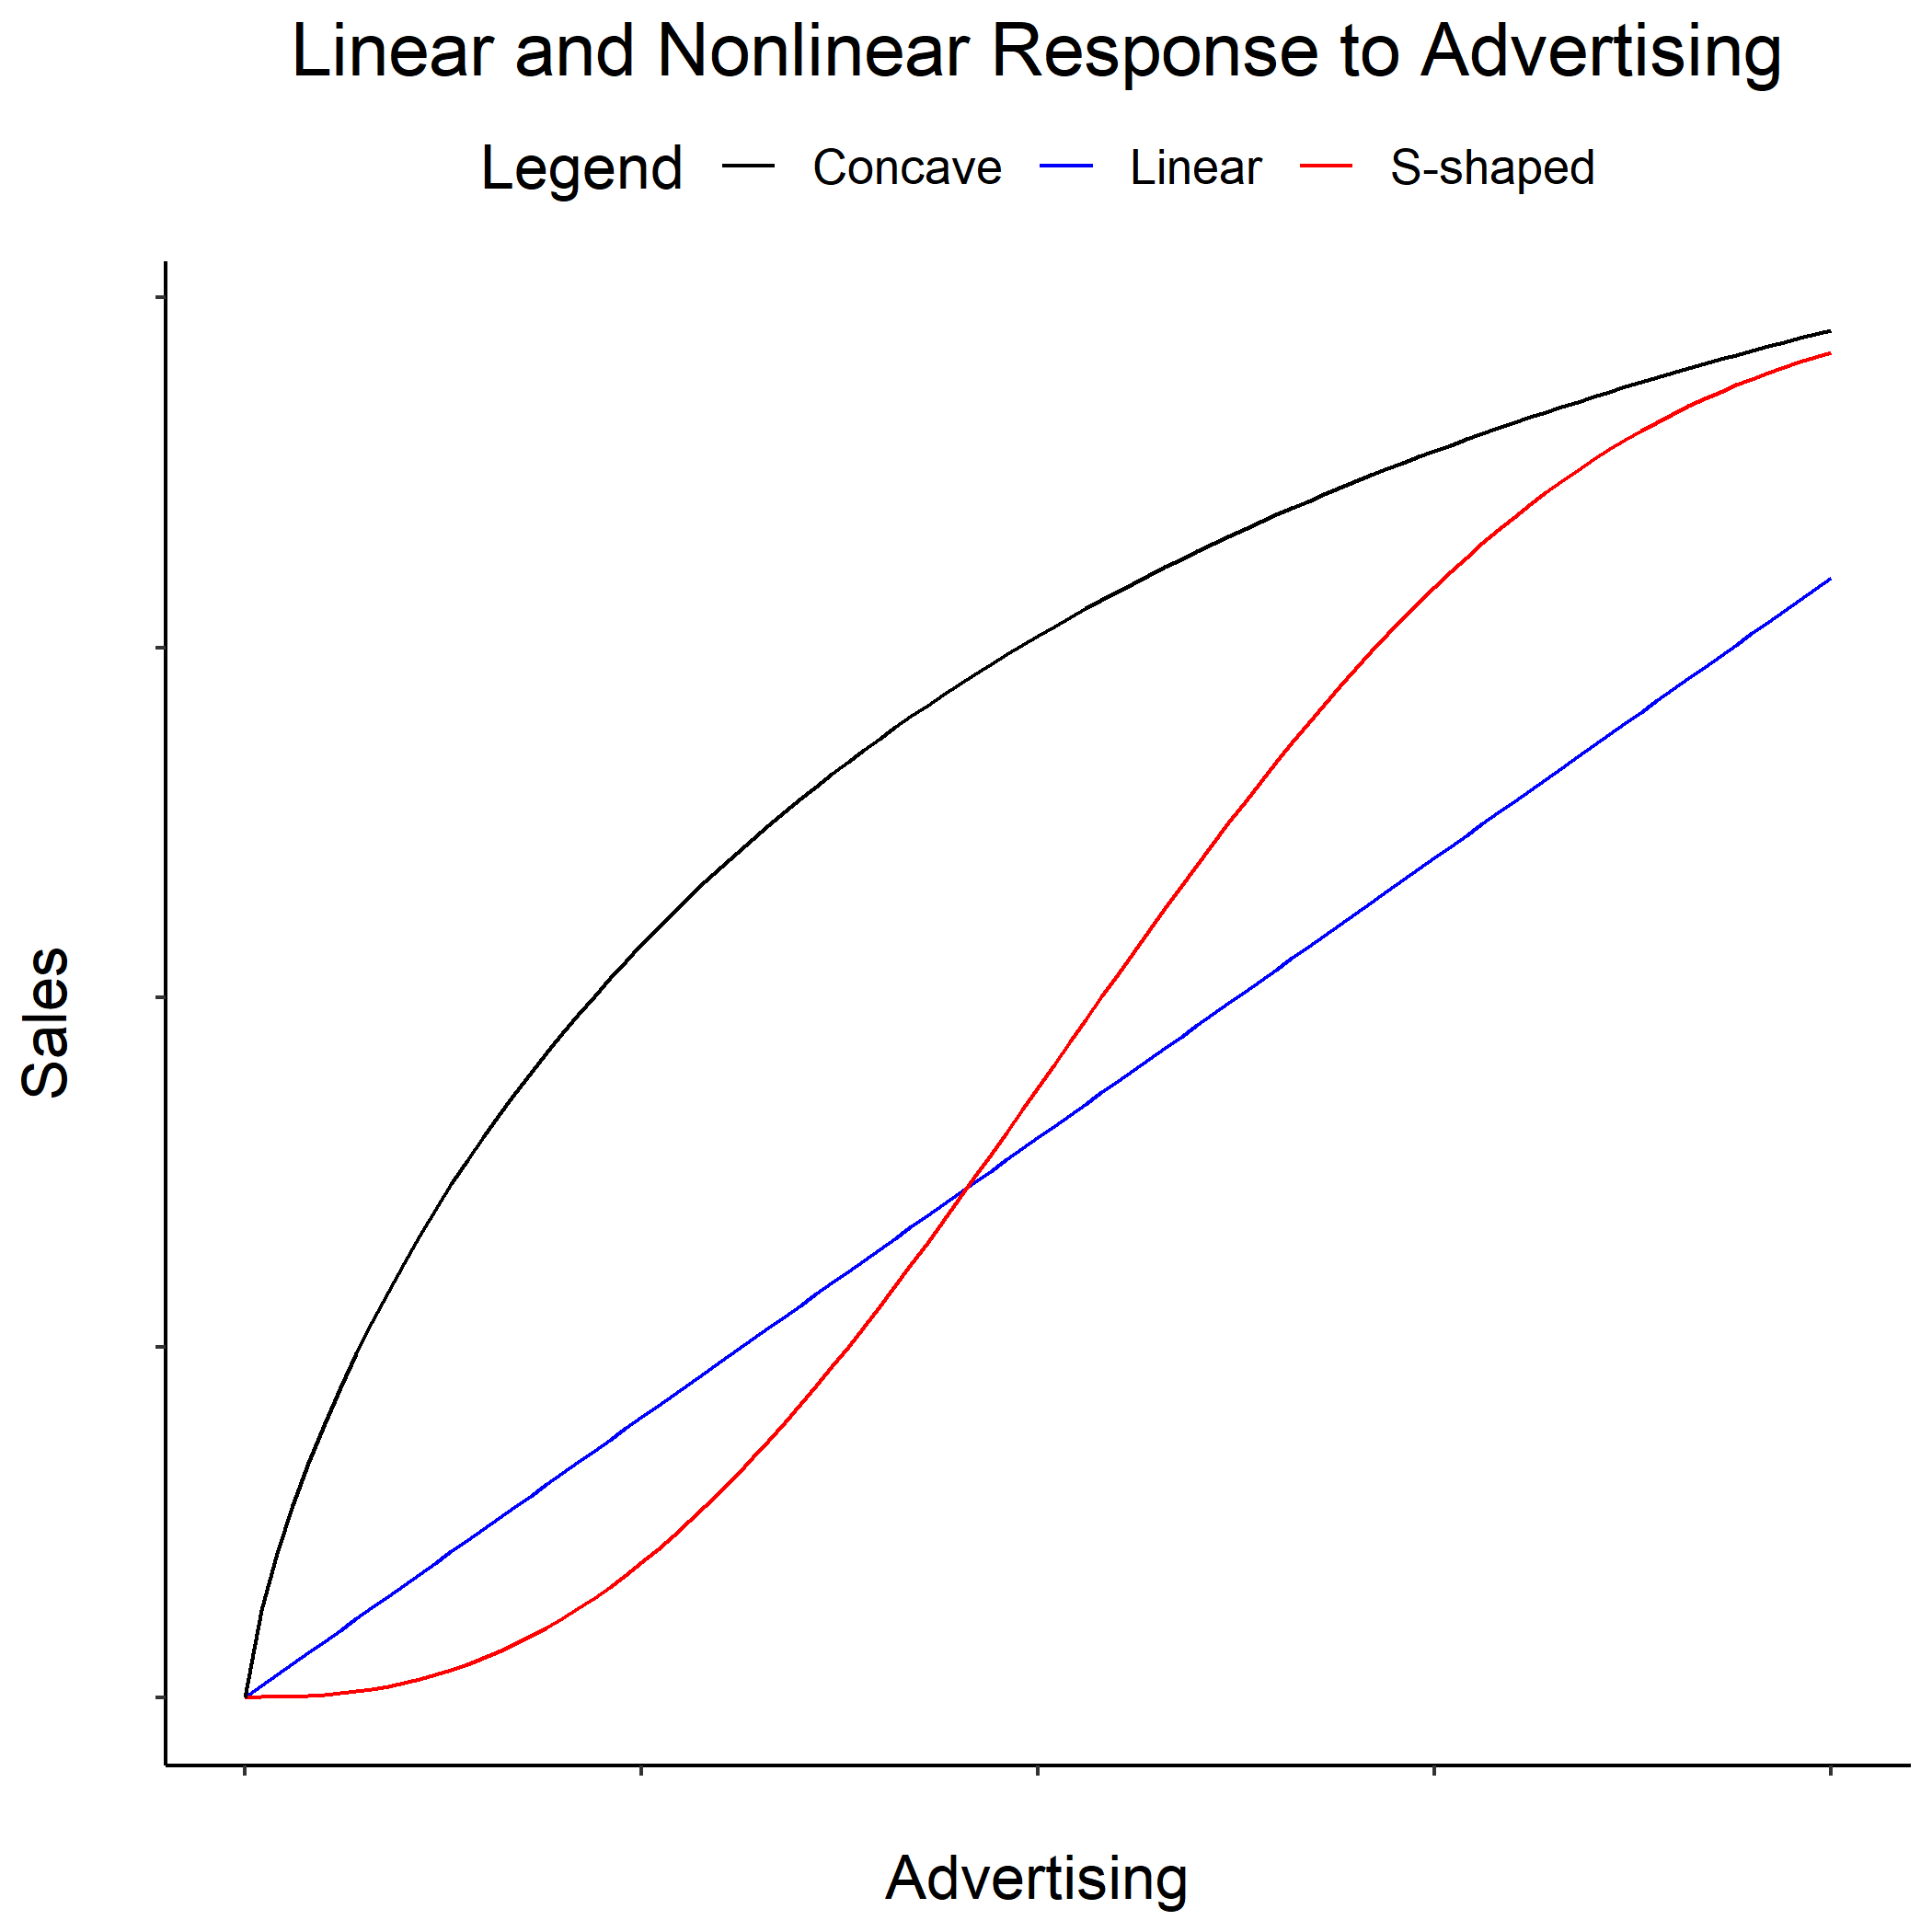
\includegraphics[height=5.0cm, trim=0.0cm 0.0cm 0.0cm 0.0cm width=5.0cm]{../BUSA_603_Ad_Response/Output/m5_a.png}
  \caption{Figure {\color{franklinblue} 11}: Linear and Nonlinear Response to Advertising}
\end{figure}
\vspace{-1.0ex}
\small
The Linear curve has constant returns to scale (CRTS), the Concave curve has decreasing returns to scale (DRTS), and the S-shaped has sections that have increasing returns to scale (IRTS) and DRTS, and an inflection point with CRTS.
\end{frame}

\section{Synergy Measurement via Linear Model Moderation}

\begin{frame}[t]{Integrated Marketing}
\empr{Integrated marketing} is an approach that uses different media channels to tell a story or convey an idea. \\
\vspace{0.0ex}
\small
\begin{itemize}
\item An integrated marketing campaign might start with a TV ad featuring a memorable character and message. The character could then appear in other channels: on billboards, on in-store displays, on coupons, in social media posts, in the original TV ad re-posted to YouTube, even in direct mail and email messages.\footnote{Coupons are a type of \empr{consumer promotion} (CP). A subdivision of a firm's marketing department typically manages CP and customer shopper marketing tactics (e.g., demonstrations, in-store radio, brand displays on shopping carts, in-store floor graphics \ldots).} 
\item By marketing their character across complementary channels, the company creates strong brand consumer awareness and association.  Thus, integrated marketing goes beyond the concurrent use of multiple media.\footnote{In the \underline{standard} multimedia approach the effectiveness of an activity does \underline{not} depend upon any other activity.}
\end{itemize} 
\end{frame}

\begin{frame}[t]{Synergy}
In integrated marketing each activity's effectiveness depends on all other brand activities. \\
\vspace{1.5ex}
\empr{Synergy} represents the joint effect of two different activities. It emerges when the combined effect of two activities exceeds the sum of their individual effects.\\
\vspace{1.5ex}
\begin{itemize}
\item Synergies may arise from combining different media types, scheduling their in-phase or out-phase timing, using consistent creative designs, and creating cross-media integrated content. 
\item As synergy increases, the optimal total media budget increases as well.  Moreover, incremental outlays should be allocated be allocated in favor of the less effective media.\footnote{For additional information see \cite{naik2003}. }
\end{itemize}
\end{frame}

\begin{frame}[t]{Moderation}
Under appropriate assumptions, the expected long-term profit of an advertised brand increases as synergy increases. Thus there are many instances where brand managers allocate a non-zero budget outlay to a catalytic activity even if it is completely ineffective.\footnote{For insights on how this result was derived, see \cite{raman2004}.}\\
\vspace{1.5ex}
For the linear model specification, synergy is measured by \empr{moderation}.  \\
\small
\begin{itemize}
  \item Moderation is enacted by including an interaction term in the linear model's specification. 
  \item An \empr{interaction} is the multiplication of two explanatory variables.\footnote{The reference article for the moderation presentation of the textbook is \cite{spiller2013}.} 
\end{itemize}
\end{frame}

\begin{frame}[t]{Synergy R\&D Continues in the Industry}
While synergy measurement is still an active area of marketing research, where much of the focus is on examining different non-linear model specifications, estimation methods, and long-term relationships, some practitioners use moderated regression to measure synergy. \\
\vspace{1.5ex}
We will illustrate moderated regression by examining the potential synergy between coupons and TV for a consumer packaged goods (CPG) brand.\footnote{A paper that attempts to measure the long-term synergy of coupons and other media is \cite{reimer2014}.  In this paper they introduce a non-moderated regression modeling approach that enables brand managers to quantify marketing effectiveness based on all available data. Their approach combines existing ``best practices'' methods of customer segmentation and long-run effects modeling to investigate marketing mix effectiveness.} 
\end{frame}


\begin{frame}[t]{Defining Numeric Distribution and ACV}
For our moderated regression specification, we will need a few definitions.\footnote{For additional details on these definitions see \cite{bendle2020}.} \\
\vspace{-0.0ex}
\small
\begin{description}
  \item[Numeric Distribution \%:] The percentage of stores that stock a given item (e.g., UPC, sub-brand, brand \ldots) within the universe of stores in the relevant market.\footnote{A \empr{relevant market} is a set of stores that have a set of common characteristics.  For example, ``Club''is a commonly examined relevant market, where the market includes \href{https://www.bjs.com/}{B.J's}, \href{https://www.costco.com/}{Costco}, and \href{https://www.samsclub.com/}{Sam's Club}.} 
  \item[All Commodity Volume (ACV):] The dollar value of store sales in \underline{all} \underline{categories} by stores in the relevant market. 
  \item [\% ACV:]  The dollar value of store sales in \underline{all} \underline{categories} by stores in the relevant market where the item is carried divided by ACV.
\end{description}
\end{frame}

\begin{frame}[t]{Defining PCV, TDPs and Velocity}
\small
  \begin{description}
  \item[Product Commodity Volume (PCV):] For a given item's category, the dollar value of \underline{category} sales by stores in the relevant market.
  \item[\% PCV:] For a given item's category, the dollar value of store \underline{category} sales by stores in the relevant market where the item is carried divided by PCV.
  \item[Total Distribution Points (TDP):]  For a given item, the sum of \% ACV of its UPCs for the relevant market.\footnote{For a detailed description, see \href{https://nielseniq.com/wp-content/uploads/sites/4/2021/02/ConnectedSystem-Job-Aid-Understanding-TDPs.pdf}{this insightful Nielsen IQ explanation}.} 
  \item[Velocity:]  An item's relevant market equivalized unit sales divided by the relevant market's ACV.   This is a  measure of how fast an item moves, controlling for differences in distribution.   
\end{description}
\end{frame}

\begin{frame}[t]{Markets Of Interest}
As the \underline{relevant market} to determine if there is synergy between coupons and TV, the CPG brand has chosen the top 20 \$2M+ ACV Grocery Chain Holding Companies.  Examples of such companies are Cincinnati-headquartered \href{https://www.thekrogerco.com/about-kroger/our-business/}{The Kroger Company} and \href{https://www.gianteagle.com/about-us/our-brands}{Giant Eagle, Inc.}  \\
\vspace{1.5ex}
The brand is from a category that does not have discernible seasonality. The Tissues Category, Laundry Detergent Category, and Men's Deodorant Categories are examples of categories that do not have pronounced seasonal effects. \\
\vspace{1.5ex}
The dependent variable of interest for the brand analysis is velocity.  The denominator, ACV, is in billions of dollars.  \\
\vspace{1.5ex}
Model dimensions are markets indexed by $m$, $m \in \{1,2,\ldots\,20\}.$ Time is measured in 4-week periods indexed by $t$, $t \in \{1,2,\ldots,26\}$.  The brand is denoted as $b$.
\end{frame}

\begin{frame}[t]{Improving the Precision of the Objective Statement}
The objective of the analysis is to determine if coupons (i.e., moderator) changes the association between national broadcast TV GRPs (i.e., the primary marketing mix modeling explanatory variable) and velocity. The coupons are market-specific (i.e., retailer-specific) promotional offers distributed through retailer-specific circulars, such as Sunday newspaper retailer inserts.  \\
\vspace{1.5ex}
We will use CPG brand household TV GRPs as the TV explanatory variable.\footnote{This models assumes the adstock retention rate is 0 and all markets receive the same number of national brand hh GRPs for a given $t$.} \\
\vspace{1.5ex}
We will use a \empr{dummy explanatory variable} to model coupons. 
\end{frame}

\begin{frame}[t]{Model Specification}
Given data available, the linear model specification is  \\
\vspace{-1.0ex}
\small
\begin{equation} \label{eq:a}
\frac{Y_{bmt}}{ACV_{mt}} = \alpha_1 + \beta_{1} x_{bt} + \gamma_1 z_{bmt} + \delta_1 x_{bt}z_{bmt} + \epsilon_{bmt},
 \end{equation}
 \normalsize
where $Y_{bmt}$ is equivalized units of $b$ in $m$ during $t$, $ACV_{mt}$ is all commodity volume of $m$ in $t$, $z_{bmt}$ is a dummy variable that is 1 if there was a coupon drop for $b$ in $m$ during $t$ and 0 otherwise, and $x_{bt}$ are national hh TV GRPs of $b$ during $t$. \\
\vspace{1.5ex}
 $ x_{bt}z_{bmt}$ is the interaction term.\\
\vspace{1.5ex}
 The errors $\epsilon_{bmt}$ are assumed to be IID, where independence is across all $m$ and all $t$.  They are assumed to be normally distributed. 
 \end{frame}

\begin{frame}[t]{Model Specification Interpretation}
To emphasize, notice that the marketing mix variable of interest, brand $b$ TV hh GRPs, and the moderator,  the coupon dummy variable, and the iteration term, enter the model specification separately. \\
\vspace{1.5ex}
In addition, it is not appropriate to include an interaction term in the model without the main effects; $x_{bt}$ and $z_{bmt}$ each entering the model specification separately.  \\
\end{frame}

\begin{frame}[t]{Importance of Moderator $p$-value}
The textbook mentions that if we are wondering whether there is evidence in the data that the association between the marketing outcome and the marketing mix variable (i.e., TV GRPs) changes depend on the moderator (i.e., retailer-specific coupons), then we just check for the significance of the interaction by examining its $p$-value.
\begin{itemize}
\item If the interaction is significant, then there is evidence that the marketing outcome's association with the marketing mix variable depends on that moderator. 
\item If it is \underline{not} significant, then we say that the marketing outcome's association
with the marketing mix variable does not depend on that moderator.
\end{itemize}
\end{frame}

\begin{frame}[t]{Model Estimation Output from the \textsf{R} \texttt{lm} Function}
\footnotesize
\verbatiminput{Images/coup_tz_reg.txt}
\end{frame}

\begin{frame}[t]{Estimated Coefficient Interpretation}
\small
The interaction is \underline{not} statistically significant. This  means that that association between the brand's TV hh GRPs and the brand's velocity do not depend on whether coupons are dropped, or not dropped, in a market.  That is, there is \underline{not} a discernible synergy effect from coupons and TV on velocity. \\
\vspace{0.5ex}
\begin{itemize}
\item $\hat{\alpha}_1$, 6589.14, is the estimate of brand velocity when brand hh TV GRPs are 0, $x_{bt} =0$, and there is \underline{not} a brand coupon drop, $z_{bmt} =0$.\\
\vspace{1.5ex}
\item $\hat{\beta}_1$, 1.19, is the simple slope of brand hh TV GRPs on brand velocity when there is \underline{not} a brand coupon drop. \\
\vspace{1.5ex}
\item $\hat{\gamma}_1$, 2682.55, is the simple effect of a brand coupon drop versus \underline{no} brand coupon drop when when brand hh TV GRPs are 0. \\
\vspace{1.5ex}
\item $\hat{\delta}_1$, 2.00, is the change in effect of the brand coupon drop versus \underline{no} brand coupon drop when hh TV GRPs increase by 1 unit.  The effect is \underline{not} statistically significant.
\end{itemize}
\end{frame}

\begin{frame}[t]{Another Moderator Regression Case Study}
 For this case study the focus is on the moderating effect of digital radio on national radio (e.g., \href{https://www.iheart.com/podcast/51-the-sean-hannity-show-24392822/}{The Sean Hannity Radio Show}).  The digital radio platforms are \href{https://www.apple.com/apple-music/}{Apple Music}, \href{https://music.amazon.com/}{Amazon Music}, \href{https://www.pandora.com/}{Pandora} and \href{https://open.spotify.com/?}{Spotify}.  \\
 \vspace{1.5ex} 
 While the company is the same as that of the previous case study, the brand is different.  Similar to the brand of the previous case study, this brand's seasonality is not pronounced. \\
\vspace{1.5ex}
While for more than a decade the brand has advertised on national radio, only during the last 3 years has the brand used digital radio advertising.  The business problems to be addressed are: \\
\vspace{0.0ex}
\small
\begin{itemize} 
\item To determine if digital radio is moderating the effectiveness of national radio.
\item If digital radio is moderating national radio, determine its magnitude. 
\end{itemize}
\end{frame}

\begin{frame}[t]{Specification of the Moderator Regression}
Given data available, the linear model specification is  \\
\vspace{-1.0ex}
\small
\begin{equation} \label{eq:a}
\frac{Y_{bt}}{ACV_{t}} = \theta_0 + \theta_1 x_{1bt} + \theta_2 x_{2bt} + \theta_3 x_{1bt}x_{2bt} + \upsilon_{bt},
 \end{equation}
 \normalsize
where $Y_{bt}$ is national equivalized units of $b$ during $t$, $ACV_{t}$ is all commodity volume of all channels in which $b$ is distributed in $t$, $x_{1bt}$ are digital radio adults aged 18 to 54 (A 18-54) impressions in millions (i.e., the moderator), and $x_{2bt}$ are national radio A 18-54 impressions in millions.\footnote{Like the previous case study's model, this simple models assumes the adstock retention rate is 0 for both radio series.} \\
\vspace{1.5ex}
 $ x_{1bt}x_{2bt}$ is the interaction term.\\
\vspace{1.5ex}
 The errors $\upsilon_{bt}$ are assumed to be IID and normally distributed.  
 \end{frame}

\begin{frame}[t]{Moderating Regression Estimates}
\footnotesize
\verbatiminput{Images/spotify_natradio_reg.txt}
\end{frame}

\begin{frame}[t]{Interpreting the Moderating Regression Results}
The above results imply that national radio A 18-54 impressions are associated with the velocity of  brand $b$, where there is dependence on digital radio A 18-54 impressions. While the interaction effect coefficient is positive and statistically significant at a significance level of 0.10, the effect of brand brand $b$ national radio on brand $b$ velocity many not be constant across all values of the moderating explanatory variable, digital radio A 18-54 impressions. \\
\vspace{1.5ex}
\empr{Spotlight analysis} compares marketing mix variable estimates across two or more values of the moderating explanatory variable.  For example, we may mean center the digital radio explanatory variable $x_{1bt}$ and re-estimate the model.  From the mean-centered value of $x_{1bt}$ we may also add or subtract 1 standard deviation (SD) and re-estimate the model to obtain other spotlights.\footnote{The interaction term is a function of the mean centered moderating explanatory variable.} 
\end{frame}

\begin{frame}[t]{Spotlighting at the Moderator's Mean}
\footnotesize
\verbatiminput{Images/spotifymc_natradio_reg.txt}
\end{frame}

\begin{frame}[t]{High-Level Spotlighting}
\footnotesize
\verbatiminput{Images/spotifynegsdc_natradio_reg.txt}
\end{frame}

\begin{frame}[t]{Low-Level Spotlighting}
\footnotesize
\verbatiminput{Images/spotifypossdc_natradio_reg.txt}
\end{frame}

\begin{frame}[t]{Interpretation of Spotlights}
The coefficient estimates of the moderating explanatory variable, $\hat{\theta}_1$, and the interaction term, $\hat{\theta}_3$, are the same for all moderating regression specifications.  This also holds for these coefficient estimates' standard errors.  This result follows from the mathematics of least squares.
\begin{description}
  \item [Spotlighting at the Moderator's Mean] When digital radio A 18-54 impressions are average, for every 1M increase in network radio A 18-54 impressions velocity increases by 57.6.
  \item [High-Level Spotlighting] When digital radio A 18-54 impressions are higher, for every 1M increase in network radio A 18-54 impressions velocity increases by 75.04.\footnote{"High" is  one standard deviation greater than the mean of digital radio A 18-54 impressions.} % Subtract 1 sd from mean centered moderator variable. 
\end{description}
\end{frame}

\begin{frame}[t]{Floodlight Analysis}
\begin{description}
    \item [Low-Level Spotlighting] When digital radio A 18-54 impressions are lower, for every 1M increase in network radio A 18-54 impressions velocity increases by 40.16.\footnote{"Low" is one standard deviation less than the mean of digital radio A 18-54 impressions.} % Add 1 sd to mean centered moderator variable.
\end{description}
\vspace{1.5ex}
\empr{Floodlight analysis} is spotlight analysis for many values across a wide range of continuous moderator variable values. \\
\vspace{1.5ex}
Spotlight analysis and floodlight analysis are useful modeling tools for marketing analytics because they allow one to examine associations between a marketing mix variable and a marketing outcome variable at different moderator variable levels.  
\end{frame}

\section{References}

\begin{frame}[t,allowframebreaks]
%https://latex-beamer.com/faq/long-bibliographies-beamer/
%https://github.com/jgm/pandoc/issues/2442
\widowpenalties 1 10000
\small
\bibliography{../../Bibliography/list2}
\bibliographystyle{apalike}
\end{frame}

\end{document}